% Template for Elsevier CRC journal article
% version 1.2 dated 09 May 2011

% This file (c) 2009-2011 Elsevier Ltd.  Modifications may be freely made,
% provided the edited file is saved under a different name

% This file contains modifications for Transportation Research Procedia

% Changes since version 1.1
% - added "procedia" option compliant with ecrc.sty version 1.2a
%   (makes the layout approximately the same as the Word CRC template)
% - added example for generating copyright line in abstract

%-----------------------------------------------------------------------------------

%% This template uses the elsarticle.cls document class and the extension package ecrc.sty
%% For full documentation on usage of elsarticle.cls, consult the documentation "elsdoc.pdf"
%% Further resources available at http://www.elsevier.com/latex

%-----------------------------------------------------------------------------------

%%%%%%%%%%%%%%%%%%%%%%%%%%%%%%%%%%%%%%%%%%%%%%%%%%%%%%%%%%%%%%
%%%%%%%%%%%%%%%%%%%%%%%%%%%%%%%%%%%%%%%%%%%%%%%%%%%%%%%%%%%%%%
%%                                                          %%
%% Important note on usage                                  %%
%% -----------------------                                  %%
%% This file should normally be compiled with PDFLaTeX      %%
%% Using standard LaTeX should work but may produce clashes %%
%%                                                          %%
%%%%%%%%%%%%%%%%%%%%%%%%%%%%%%%%%%%%%%%%%%%%%%%%%%%%%%%%%%%%%%
%%%%%%%%%%%%%%%%%%%%%%%%%%%%%%%%%%%%%%%%%%%%%%%%%%%%%%%%%%%%%%

%% The '3p' and 'times' class options of elsarticle are used for Elsevier CRC
%% The 'procedia' option causes ecrc to approximate to the Word template
\documentclass[3p,times,procedia]{elsarticle}
\flushbottom

%% The `ecrc' package must be called to make the CRC functionality available
\usepackage{ecrc}
%\usepackage{amsmath}


%%%%%%%%%%


%%%%%
% variable to include comments or not in the compilation ; set to 1 to include
\def \draft {1}
%\def \draft {0}


% writing utilities

% comments and responses
%  -> use this comment to ask questions on what other wrote/answer questions with optional arguments (up to 4 answers)
\usepackage{xparse}
\usepackage{ifthen}
\DeclareDocumentCommand{\comment}{m o o o o}
{\ifthenelse{\draft=1}{
    \textcolor{red}{\textbf{C : }#1}
    \IfValueT{#2}{\textcolor{blue}{\textbf{A1 : }#2}}
    \IfValueT{#3}{\textcolor{ForestGreen}{\textbf{A2 : }#3}}
    \IfValueT{#4}{\textcolor{red!50!blue}{\textbf{A3 : }#4}}
    \IfValueT{#5}{\textcolor{Aquamarine}{\textbf{A4 : }#5}}
 }{}
}


% todo
\newcommand{\todo}[1]{
\ifthenelse{\draft=1}{\textcolor{red!50!blue}{\textbf{TODO : \textit{#1}}}}{}
}

\makeatletter
\makeatother

\usepackage{color}





%% The ecrc package defines commands needed for running heads and logos.
%% For running heads, you can set the journal name, the volume, the starting page and the authors

%% set the volume if you know. Otherwise `00'
\volume{00}

%% set the starting page if not 1
\firstpage{1}

%% Give the name of the journal
\journalname{Transportation Research Procedia}

%% Give the author list to appear in the running head
%% Example \runauth{C.V. Radhakrishnan et al.}
\runauth{Raimbault and Bergeaud}

%% The choice of journal logo is determined by the \jid and \jnltitlelogo commands.
%% A user-supplied logo with the name <\jid>logo.pdf will be inserted if present.
%% e.g. if \jid{yspmi} the system will look for a file yspmilogo.pdf
%% Otherwise the content of \jnltitlelogo will be set between horizontal lines as a default logo

%% Give the abbreviation of the Journal.
\jid{aaspro}

%% Give a short journal name for the dummy logo (if needed)
%\jnltitlelogo{Transportation Research Procedia}

%% Hereafter the template follows `elsarticle'.
%% For more details see the existing template files elsarticle-template-harv.tex and elsarticle-template-num.tex.

%% Elsevier CRC generally uses a numbered reference style
%% For this, the conventions of elsarticle-template-num.tex should be followed (included below)
%% If using BibTeX, use the style file elsarticle-num.bst

%% End of ecrc-specific commands
%%%%%%%%%%%%%%%%%%%%%%%%%%%%%%%%%%%%%%%%%%%%%%%%%%%%%%%%%%%%%%%%%%%%%%%%%%

%% The amssymb package provides various useful mathematical symbols

\usepackage{amssymb}
%% The amsthm package provides extended theorem environments
%% \usepackage{amsthm}

%% The lineno packages adds line numbers. Start line numbering with
%% \begin{linenumbers}, end it with \end{linenumbers}. Or switch it on
%% for the whole article with \linenumbers after \end{frontmatter}.
%% \usepackage{lineno}

%% natbib.sty is loaded by default. However, natbib options can be
%% provided with \biboptions{...} command. Following options are
%% valid:

%%   round  -  round parentheses are used (default)
%%   square -  square brackets are used   [option]
%%   curly  -  curly braces are used      {option}
%%   angle  -  angle brackets are used    <option>
%%   semicolon  -  multiple citations separated by semi-colon
%%   colon  - same as semicolon, an earlier confusion
%%   comma  -  separated by comma
%%   numbers-  selects numerical citations
%%   super  -  numerical citations as superscripts
%%   sort   -  sorts multiple citations according to order in ref. list
%%   sort&compress   -  like sort, but also compresses numerical citations
%%   compress - compresses without sorting
%%
\biboptions{authoryear}

% \biboptions{}

% if you have landscape tables
\usepackage[figuresright]{rotating}
%\usepackage{harvard}
% put your own definitions here:x
%   \newcommand{\cZ}{\cal{Z}}
%   \newtheorem{def}{Definition}[section]
%   ...

% add words to TeX's hyphenation exception list
%\hyphenation{author another created financial paper re-commend-ed Post-Script}

% declarations for front matter

\begin{document}

\begin{frontmatter}

%% Title, authors and addresses

%% use the tnoteref command within \title for footnotes;
%% use the tnotetext command for the associated footnote;
%% use the fnref command within \author or \address for footnotes;
%% use the fntext command for the associated footnote;
%% use the corref command within \author for corresponding author footnotes;
%% use the cortext command for the associated footnote;
%% use the ead command for the email address,
%% and the form \ead[url] for the home page:
%%
%% \title{Title\tnoteref{label1}}
%% \tnotetext[label1]{}
%% \author{Name\corref{cor1}\fnref{label2}}
%% \ead{email address}
%% \ead[url]{home page}
%% \fntext[label2]{}
%% \cortext[cor1]{}
%% \address{Address\fnref{label3}}
%% \fntext[label3]{}

\dochead{20th EURO Working Group on Transportation Meeting, EWGT2017, 4-6 September 2017, Budapest, Hungary}
%% Use \dochead if there is an article header, e.g. \dochead{Short communication}
%% \dochead can also be used to include a conference title, if directed by the editors
%% e.g. \dochead{17th International Conference on Dynamical Processes in Excited States of Solids}

\title{The Cost of Transportation : Spatial Analysis of US Fuel Prices}

%% use optional labels to link authors explicitly to addresses:
%% \author[label1,label2]{<author name>}
%% \address[label1]{<address>}
%% \address[label2]{<address>}



\author[a,b]{Juste Raimbault\corref{cor1}}
\author[c,d]{Antonin Bergeaud}

\address[a]{UMR CNRS 8504 G{\'e}ographie-cit{\'e}s, 13 rue du Four, Paris, France}
\address[b]{UMR-T IFSTTAR 9403 LVMT, Cit{\'e} Descartes, Champs-sur-Marne, France}
\address[c]{Banque de France, Paris, France}
\address[d]{Paris School of Economics - EHESS, Paris, France}


\begin{abstract}
The geography of fuel prices has several implications, from a significant impact on accessibility patterns to issues of territorial equity and transportation governance. In this paper, we study its spatio-temporal patterns at a high resolution. We construct a dataset collecting daily oil prices for two months, on a significant proportion of US gaz facilities, using a specifically-designed large scale data crawling technology. The implementation of a web-application for interactive spatio-temporal data exploration guide further statistical investigations, namely that oil price exhibit patterns that are strongly non-stationary in space and time. The behavior of spatial autocorrelation suggests the use of specific spatial econometric methods to study the role of explanatory variables that are either geographical or temporal. We study the influence of socio-economic variables, by using complementary methods: Geographically Weighted Regression to take into account spatial non-stationarity, and Multi-level modeling to condition both at the state and county level. The former yields an optimal spatial range roughly corresponding to stationarity scale, and significant influence of variables such as population density or median income, but is less accurate around administrative borders. On the other hand, multi-level modeling reveals a strong state fixed effect, and also a non-negligible county effect. Through the combination of such methods, we unveil the superposition of a governance process with a local socio-economical spatial process. Results are furthermore consistent across the different dates. We discuss one important application that is the elaboration of locally parametrized car-regulation policies.
\end{abstract}

\begin{keyword}
Fuel Price \sep Data Crawling \sep Spatial Analysis \sep Geographically Weighted Regression \sep Multi-level Modeling
\end{keyword}


\cortext[cor1]{Corresponding author. Tel.: +0-000-000-0000 ; fax: +0-000-000-0000.}
\end{frontmatter}

%\correspondingauthor[*]{Corresponding author. Tel.: +0-000-000-0000 ; fax: +0-000-000-0000.}
\email{juste.raimbault@polytechnique.edu}



%%
%% Start line numbering here if you want
%%
% \linenumbers





%% main text

%\enlargethispage{-7mm}



%%%%%%%%%%%%%%%%%%%%%%
\section{Introduction}
\label{main}

What drives the price of fuel? Using a new database on oil price at a gas station level collected during two months, we explore its variability across time and space. Variation in the cost of fuel can have many causes, from the crude oil price to local tax policy and geographical features, all having heterogeneous effect in space and time. If the evolution of the average fuel price in time is an indicator that is carefully followed and analyzed by many financial institution, its variability across space remain a rather unexplored topic in the literature. Yet, such differences can reflect variation in more indirect socio-economic indicators such as territorial inequalities and geographical singularities or consumer preferences.

%The local cost of fuel is the outcome of heterogeneous processes at multiple scales, from raw oil prices to governance processes inducing taxes and economic interests of various agents including retail companies and consumer. If its variability in time is an evidence, the question of its variability in space has been poorly tackled in the literature, although it may have several empirical applications such as unveiling territorial inequalities, geographical singularities, or serving as a proxy of a socio-economical status, but also practical application such as a higher level of transparency for the consumer or a possible feedback of prices analyses on the process itself (regulation through increased information).

There exists to our knowledge no systematic mapping in space and time of retail fuel prices for a country. The main reason is probably that the availability of data have been a significant obstacle. It is also likely that the nature of the problem may also have influence, as it lies at the crossroad of several disciplines. While economists study price elasticity and measurement in different markets, transportation geography with method such as transportation prices in spatialized models, puts more emphasis on spatial distribution than on precise market mechanisms. Nevertheless, examples of somehow related works can be found. For example,~\cite{rietveld2001spatial} studies the impact of cross-border differences in fuel price and the implications for gradual spatial taxation in  Netherlands. At the country-level, \cite{rietveld2005fuel} provides statistical models to explain fuel price variability across European countries. \cite{macharis2010decision} models the impact of spatial fuel price variation on patterns of inter-modality, implying that the spatial heterogeneity of fuel prices has a strong impact on user behavior. With a similar view on the geography of transportation, \cite{gregg2009temporal} studies spatial distribution of gas emission at the US-state level. The geography of fuel prices also have important implications on effective costs, as shows \cite{combes2005transport} by determining accurate transportation costs across urban areas for France. More closely related to our work, and using very similar daily open data for France, \cite{gautier2015dynamics} investigate dynamics of transmission from crude oil prices to fuel retail prices. However, they do not introduce an explicit spatial model of prices diffusion and do not study spatio-temporal dynamics. 

In this paper we take the analysis one step further by proceeding to exploratory spatial analysis on US fuel prices. 

to unveil possible spatial patterns and how they can link to socio-economic properties.


%%%%
% More biblio à lire/trier :

% https://www.osti.gov/scitech/biblio/401732
% http://www.sciencedirect.com/science/article/pii/S0301421511002904
% http://onlinelibrary.wiley.com/doi/10.1111/1467-6451.00059/epdf
% http://download.springer.com/static/pdf/757/chp%253A10.1007%252F978-3-540-69170-9_10.pdf?originUrl=http%3A%2F%2Flink.springer.com%2Fchapter%2F10.1007%2F978-3-540-69170-9_10&token2=exp=1488029734~acl=%2Fstatic%2Fpdf%2F757%2Fchp%25253A10.1007%25252F978-3-540-69170-9_10.pdf%3ForiginUrl%3Dhttp%253A%252F%252Flink.springer.com%252Fchapter%252F10.1007%252F978-3-540-69170-9_10*~hmac=24266edff972aec8557505c5eb69de38e933b473e2b8ab37cd081e588fc33903
% http://www.sciencedirect.com/science/article/pii/S0966692300000454



The rest of the paper is organized as follows: in the next section, we describe a generic procedure and the tool used for a systematic data collection. We also present our dataset. In section \ref{sec:result} we conduct statistical analysis in order to study the spatio-temporal variation of fuel price and test the potential correlation with some covariates. Finally, in section \ref{sec:discuss} we discuss our results and conclude.

%%%%%%%%%%%%%%%%%%%%%%
\section{Dataset} \label{sec:data}
%%%%%%%%%%%%%%%%%%%%%%
HOW MANY GAS STATION IN THE US? COMPARED TO OUR DATASET
\subsection{Collecting large scale heterogeneous data}

The availability of new type of data has induced consequent changes in various disciplines from social science (e.g. online social network analysis~\cite{tan2013social}) to geography (e.g. new insights into urban mobility or perspectives on ``smarter'' cities~\cite{batty2013big}) and economics where the availability of exhaustive individual or firm level data is seen as a revolution. Study involving these new data are not always easy to situate or legitimate at the interface of implied disciplines, as shows the example of the difficult understanding between physics and urban sciences mentioned in \cite{dupuy2015sciences}. 

Collection and use of new data has therefore become a crucial task in social-science. 

The construction of such datasets is however far from straightforward, as their analyses because of the incomplete and noisy nature of data. Specific technical tools have to be implemented, often with a problem-specific tuning making them difficultly generic. We develop such a tool that fills the following constraints typical of large scale data collection: (i) reasonable level of flexibility and genericity; (ii) performance optimized, through parallel collection jobs; (iii) anonymity of collection jobs to avoid any possible bias in the behavior of the data source. The architecture, at a high level, has the following structure:
\begin{itemize}
\item An independent pool of tasks runs continuously socket proxies to pipe requests through \texttt{tor}.
\item A manager monitors current collection tasks, split collection between subtasks and launches new ones when necessary.
\item Subtasks can be any callable application taken as argument destination urls, they proceed to the crawling, parsing and storage of collected data.
\end{itemize}
The application is open and its module are reusable: source code is available on the repository of the project\footnote{at \texttt{https://github.com/JusteRaimbault/EnergyPrice}}.




%%%%%%%%%%%%%%%%%%%%%%
\subsection{Dataset}

%\comment{(Juste) on ne mettra pas le dataset public dans un premier temps, voir ce que les reviewers en disent}
%\comment{information density map as supplementary material ?} -> not necessary

Our dataset of fuel prices consists in crowdsourced information of retail fuel prices from various web sources. These information are aggregated with the above-described crawling tool. The dataset comprises around $41\cdot 10^6$ unique observations, spanning in time from 2017-01-10 to 2017-03-19 and corresponds to 118,573 unique retail stations. For each of these stations, we associate a precise geographical location (city resolution). On average we have XX information by station. 



Prices correspond to an unique purchase mode (credit card, other modes such as cash being less than 10\% in test datasets, they were discarded in the final dataset) and four fuel types: Diesel (18\% of observations), Regular (34\%), Midgrade (24\%) and Premium (24\%). The best coverage of stations is for Regular fuel type (\comment{recompute proportion on full dataset}), and we choose to work with this one in our exploratory analysis, keeping in mind that further developments with the dataset may include comparative analysis on fuel types.


\comment{Aggregate on which time span ? best is to check time to converge to a certain coverage of all stations (say 95\%) $\rightarrow$ around one week seems ok (see stations count plot in repo)}

\comment{French Open Data : https://www.prix-carburants.gouv.fr/rubrique/opendata/ $\rightarrow$ look to what extent our study could be transfered to France}

The socio-economic data we use are basic population and job related variables (namely income, population, jobs, wage per job, jobs per capita), available from the US Census Bureau. We use the latest available, aggregated at the county level.



%%%%%%%%%%%%%%%%%%%%%%
\section{Results} \label{sec:result}
%%%%%%%%%%%%%%%%%%%%%%


%%%%%%%%%%%%%%%%%%%%%%
\subsection{Spatio-temporal Patterns of Prices}\label{subsec:patterns}


Before moving to a more systematic study of the variation of fuel price, we propose a first exploratory introduction to give insight about its spatio-temporal structure. This exercise is a crucial stage to guide further analyses, but also to understand their implications in a geographical context. 



A lightweight web application for interactive exploration in space and time was implemented for that purpose, and is available at \texttt{}.


%%%%%%%%%%%%%%%%%%%%%%
\begin{figure}
\centering
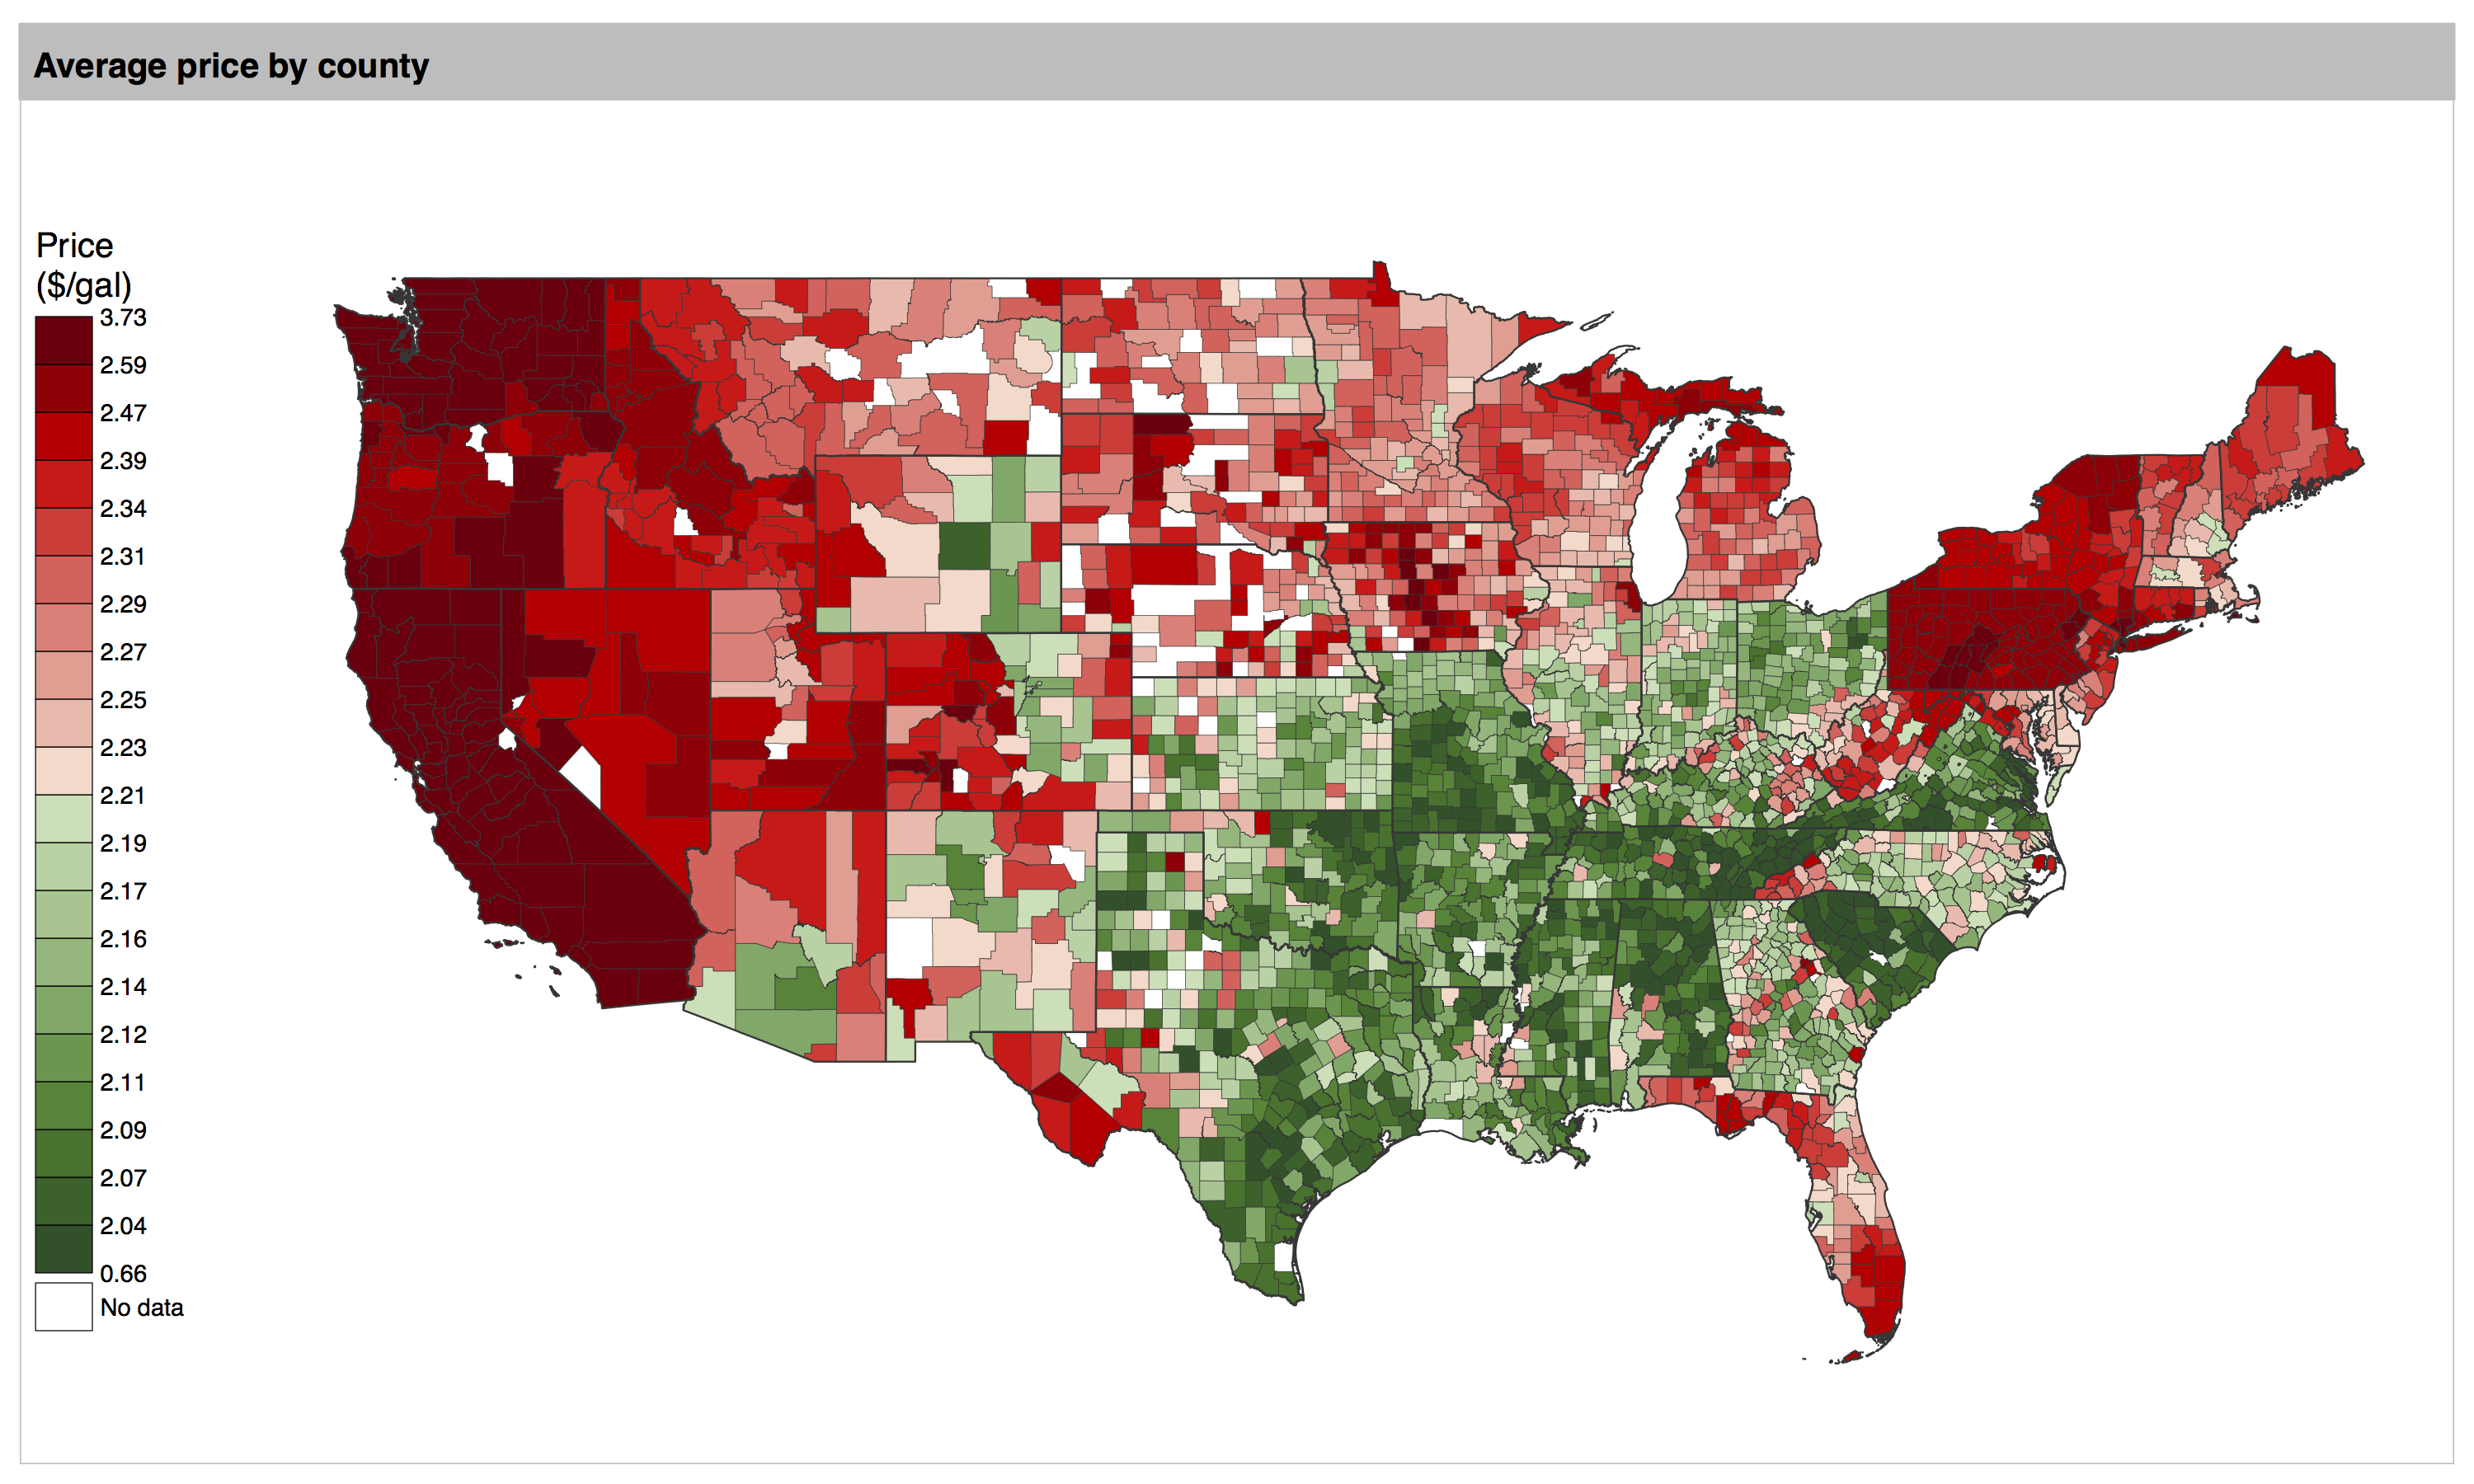
\includegraphics[width=\textwidth]{figures/average_regular_map}
\caption{Map of mean price for counties, regular fuel, averaged over the whole period.}
\end{figure}
%%%%%%%%%%%%%%%%%%%%%%


%%%%%%%%%%%%%%%%%%%%%%
\subsection{Spatial Autocorrelation}


We now turn to the study of spatial autocorrelation of prices, which can be seen as an indicator of spatial heterogeneity. We use the Moran index~(\cite{tsai2005quantifying}), with spatial weights of the form $\exp{\left(-d_{ij} / d_0 \right)}$ with $d_{ij}$ being the distance between spatial entities $i$ and $j$, and $d_0$ a decay parameter giving the spatial range of interactions taken into account in the computation. We show in Fig.~\ref{fig:moran} its variations in time and as a function of decay parameter. 
The fluctuations in time of the daily Moran index for low and medium spatial range, confirms geographical particularities in the sense of locally changing correlation regimes. These are logically smoothed for long ranges, as price correlations drop down with distance. The behavior of spatial autocorrelation with decay distance is particularly interesting: we observe a first regime change around 10km (from constant to piecewise linear regime), and a second important one around 1000km, both consistent across weekly time windows. We postulate that these correspond to typical spatial scales of the involved processes: the low regime would be local specificities and the middle one the state level processes. This behavior confirms that prices are non-stationary in space, and that therefore appropriate statistical techniques must be used to study potential drivers. The two next subsections follow this idea and investigate potential explicative variables of local fuel prices, using two different techniques corresponding to two complementary paradigms: geographically weighted regression that puts the emphasis on neighborhood effects, and multi-level regression taking into account administrative boundaries.



%%%%%%%%%%%%%%%%%%%%%%
\begin{figure}
\centering
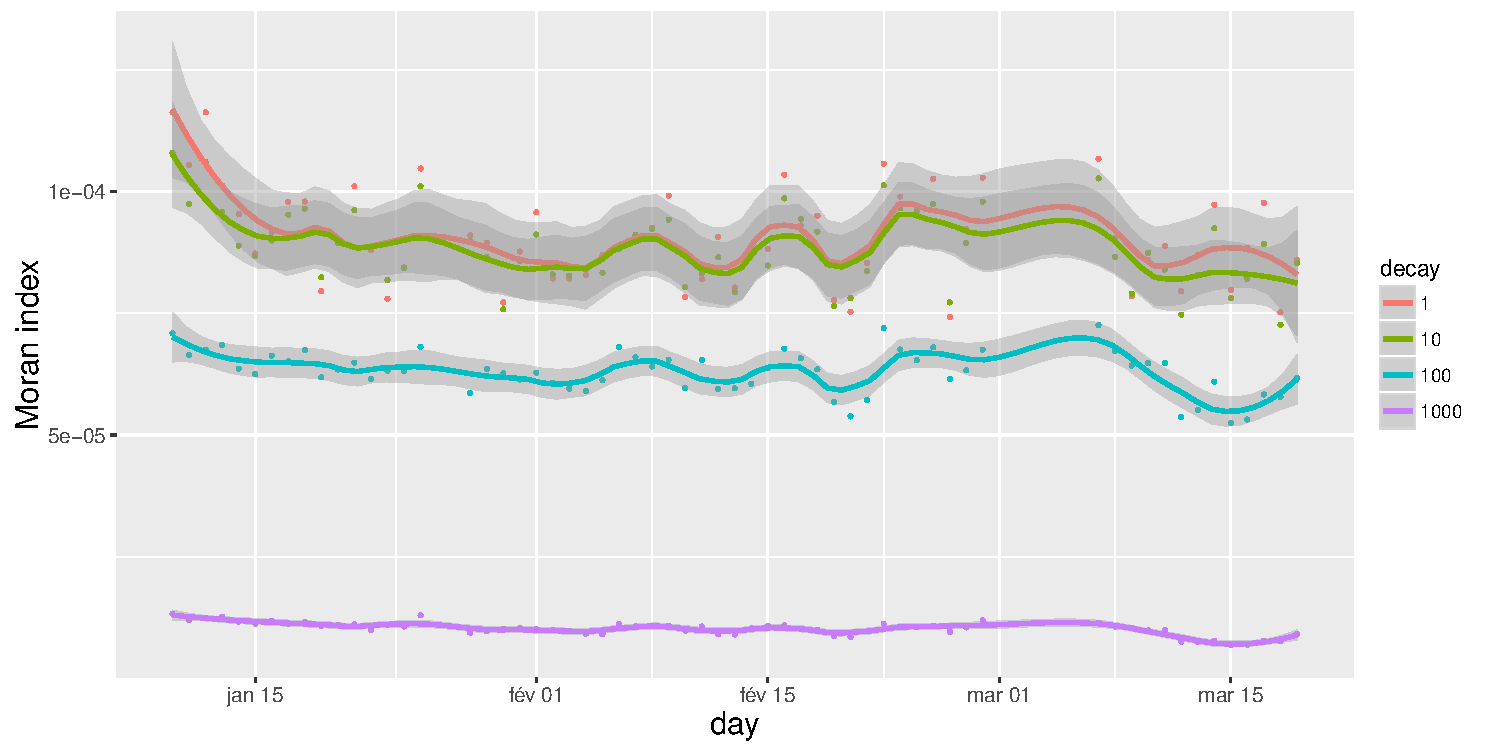
\includegraphics[width=0.48\textwidth]{figures/moran_days}
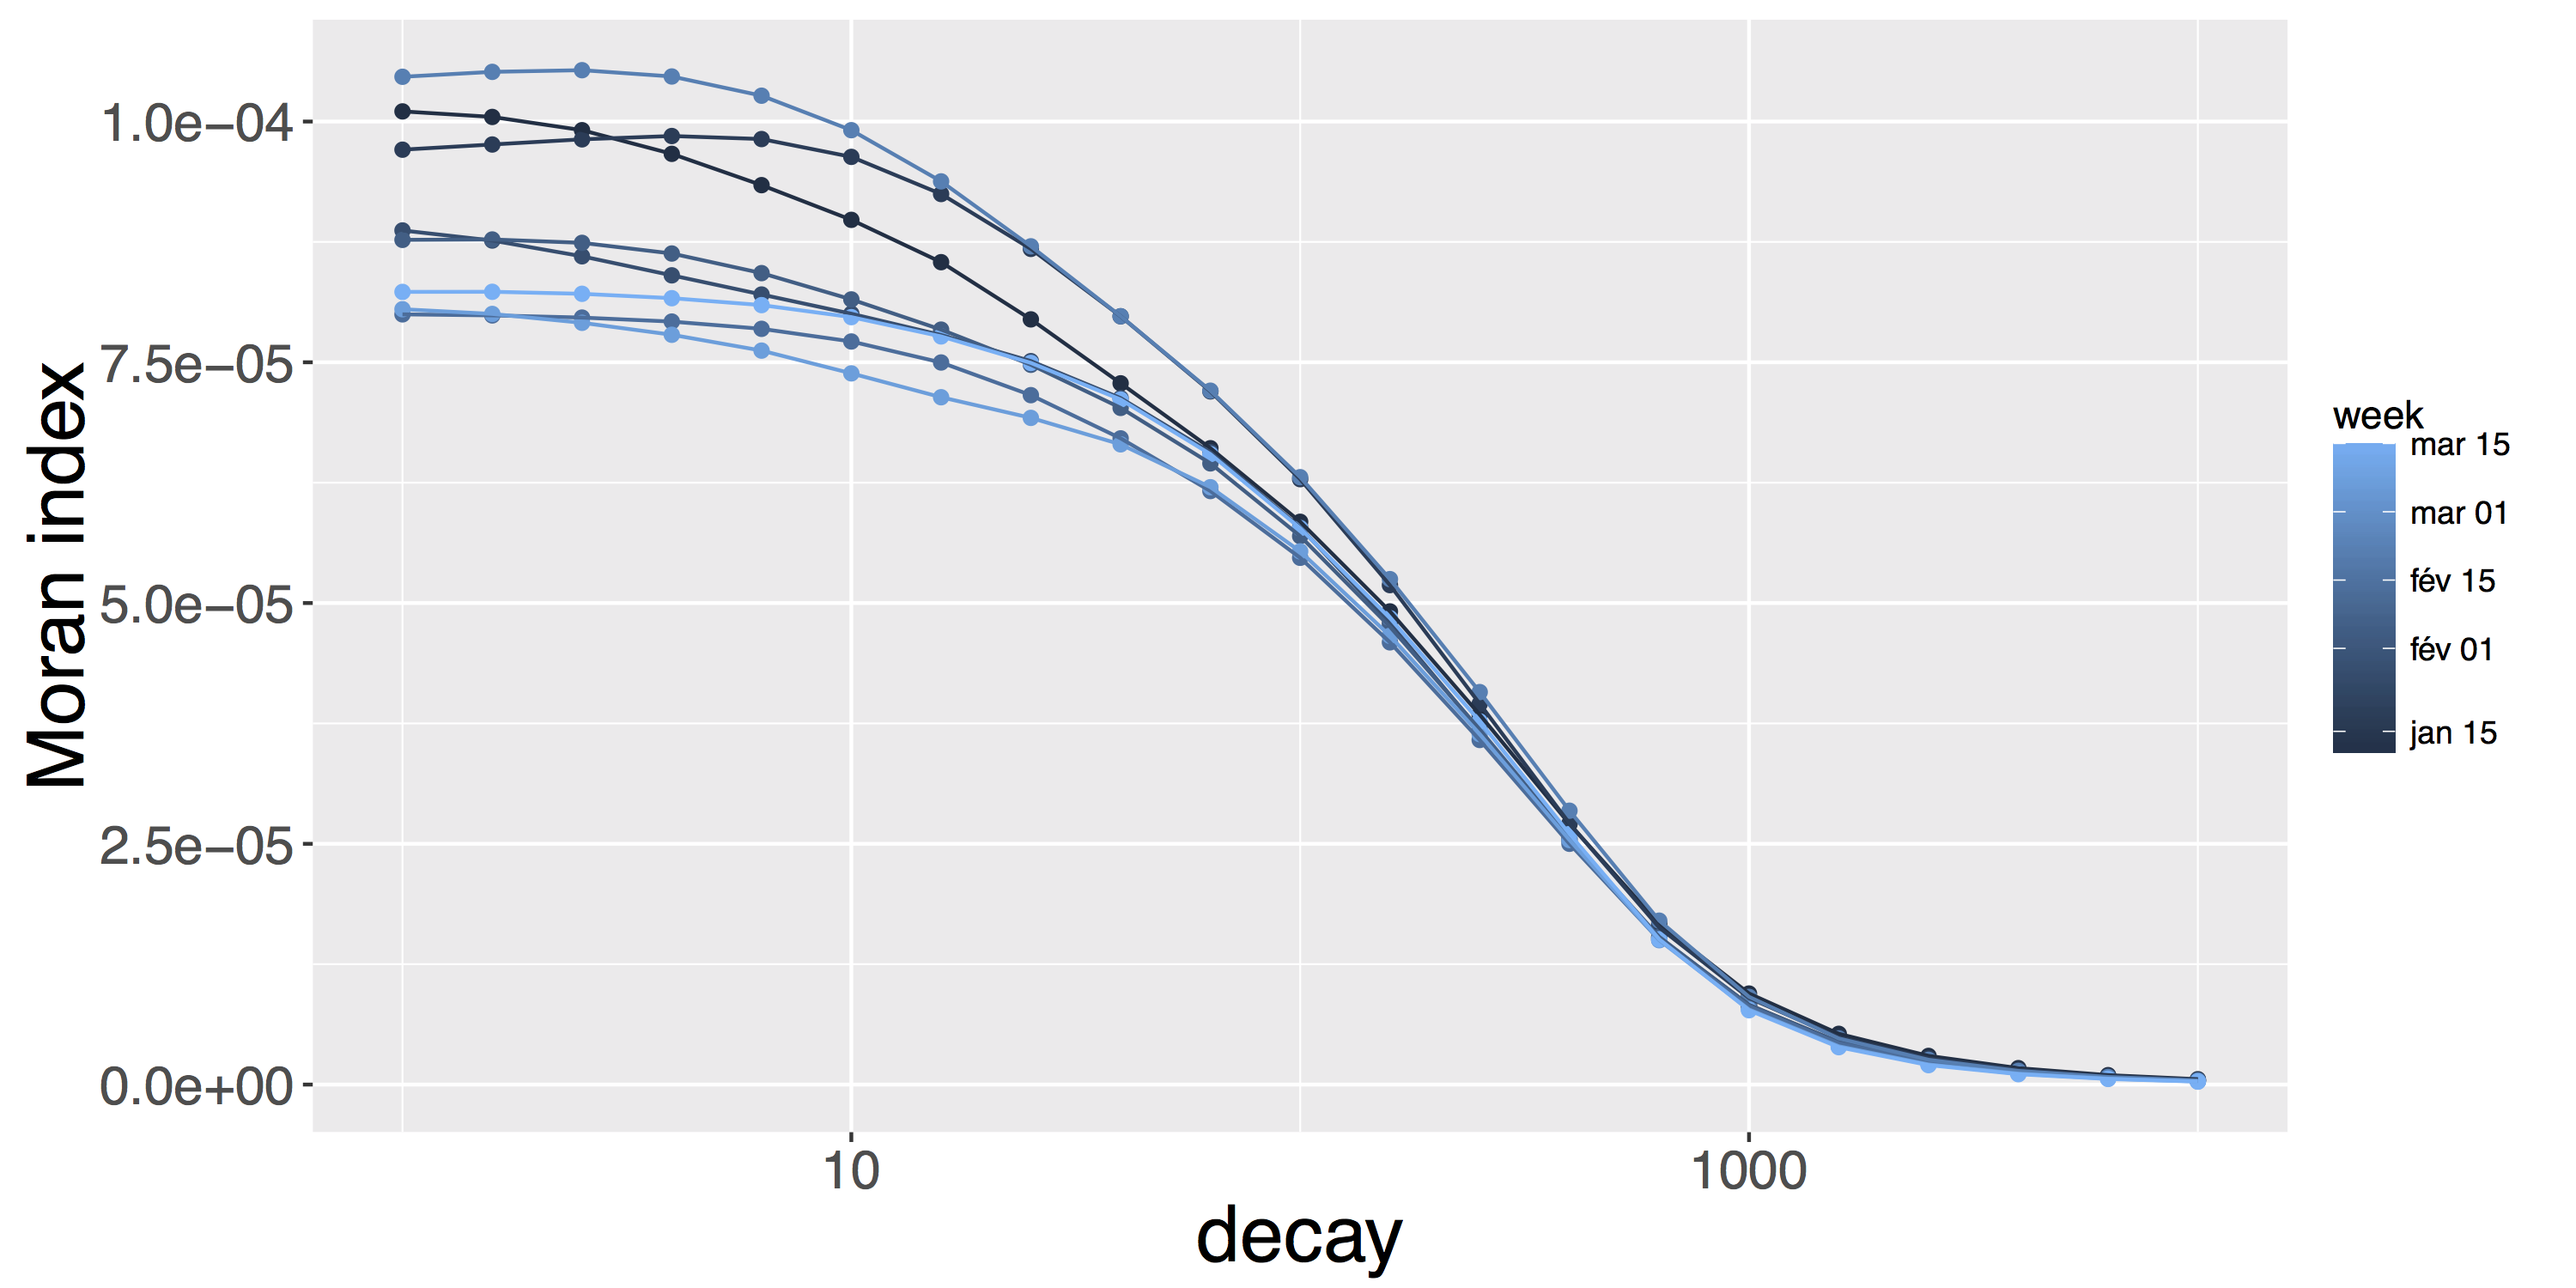
\includegraphics[width=0.48\textwidth]{figures/moran_decay_weeks}
\caption{\textbf{Behavior of Moran spatial-autocorrelation index.} (Left) Evolution in time of Moran index computed on daily time windows, for different decay parameter values. (Right) Moran index as a function of decay parameter, computed on weekly time windows.}
\label{fig:moran}
\end{figure}
%%%%%%%%%%%%%%%%%%%%%%




%%%%%%%%%%%%%%%%%%%%%%
\subsection{Geographically Weighted Regression}

The issue of spatial non-stationarity of geographical processes has always been a source of biased aggregated analyses or misinterpretations when applying general conclusions to local cases. To take it into account into statistical models, numerous techniques have been developed, among which the simple but very elegant Geographically Weighted Regression, that estimates non-stationary regressions by weighting observations in space similarly to kernel estimation methods. It was introduced in a seminal paper by~\cite{brunsdon1996geographically} and has been consequently used and matured since. The significant advantage of this technique is that an optimal spatial range in the sense of model performance can be inferred, and that the corresponding model gives effect of variables varying in space, revealing thus local effects that can occur at different spatial scales or across boundaries. We proceed to multi-modeling to find the best model and associated kernel and spatial range. The workflow is the following: (i) we generate all possible linear models from the five potential variables (income, population, wage per job, jobs per capita, jobs); (ii) for each model and each candidate kernel shape (exponential, gaussian, bisquare, step), we determine the optimal bandwidth in the sense of both cross-validation and corrected Akaike Information Criterion (AICc) which quantifies information included in the model, taking into account both model fit and number of parameters to avoid overfitting; (iii) models are fitted with this bandwidth. We choose the model with the best overall AICc, namely $price = \beta\cdot\left( income, wage, percapjobs\right)$ for a bandwidth of 22 neighbors and a gaussian kernel\footnote{note that the kernel }, with an AICc of $2900$. The median AICc difference with all other models tested is 122. The global r-squared is 0.27, what is relatively good also compared to the best r-squared of 0.29 (obtained for the model with all variables, which clearly overfits with an AICc of 3010; furthermore, effective dimension is less than 5 as 90\% of variance is explained by the three first principal components for the normalized variables). The coefficients and local r-squared for this model are shown in Fig.~\ref{fig:gwr}. The spatial distribution of residuals (not shown here) seems globally random, which confirms in a way the consistency of the approach: if a distinguishable geographical structure is found in residuals, it means that the geographical model or the variable taken into account fail to translate spatial structure.


% - similarity with corssvalidation bandwidth ? 
%  - distance range corresponding to bandwidth ?


%%%%%%%%%%%%%%%%%%%%%%
\begin{figure}
\centering
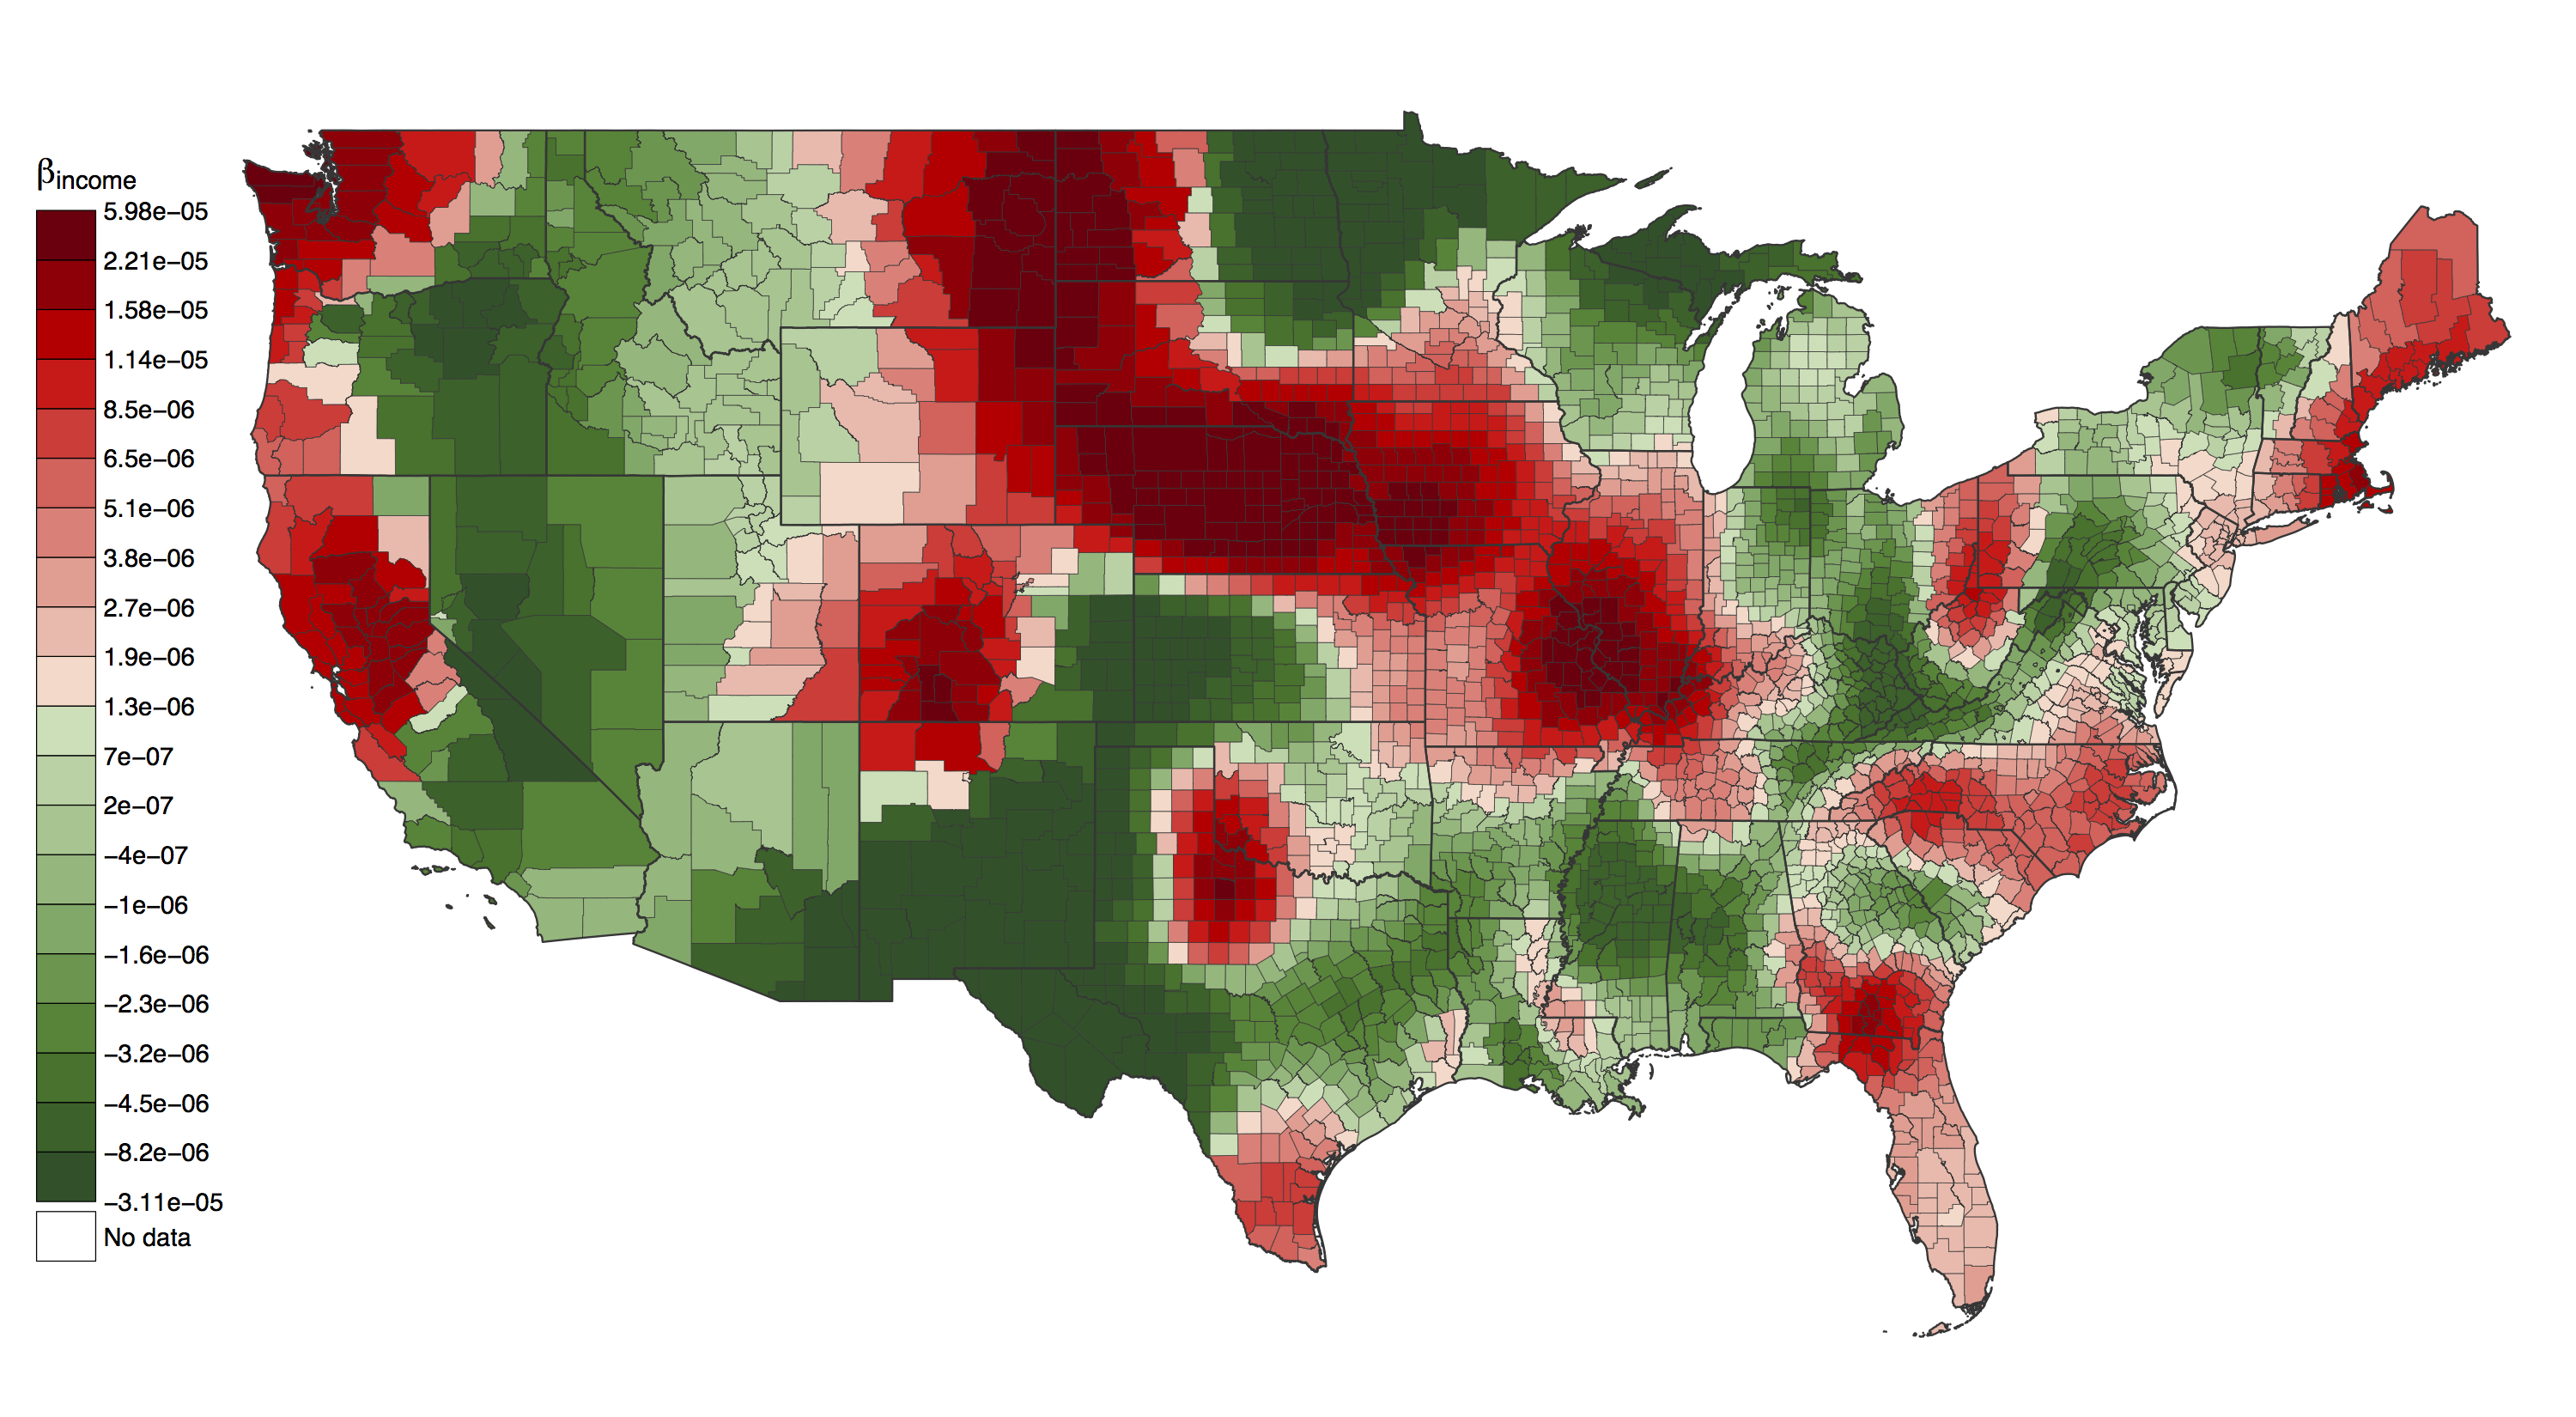
\includegraphics[width=0.48\textwidth]{figures/gwr_allbest_betaincome}
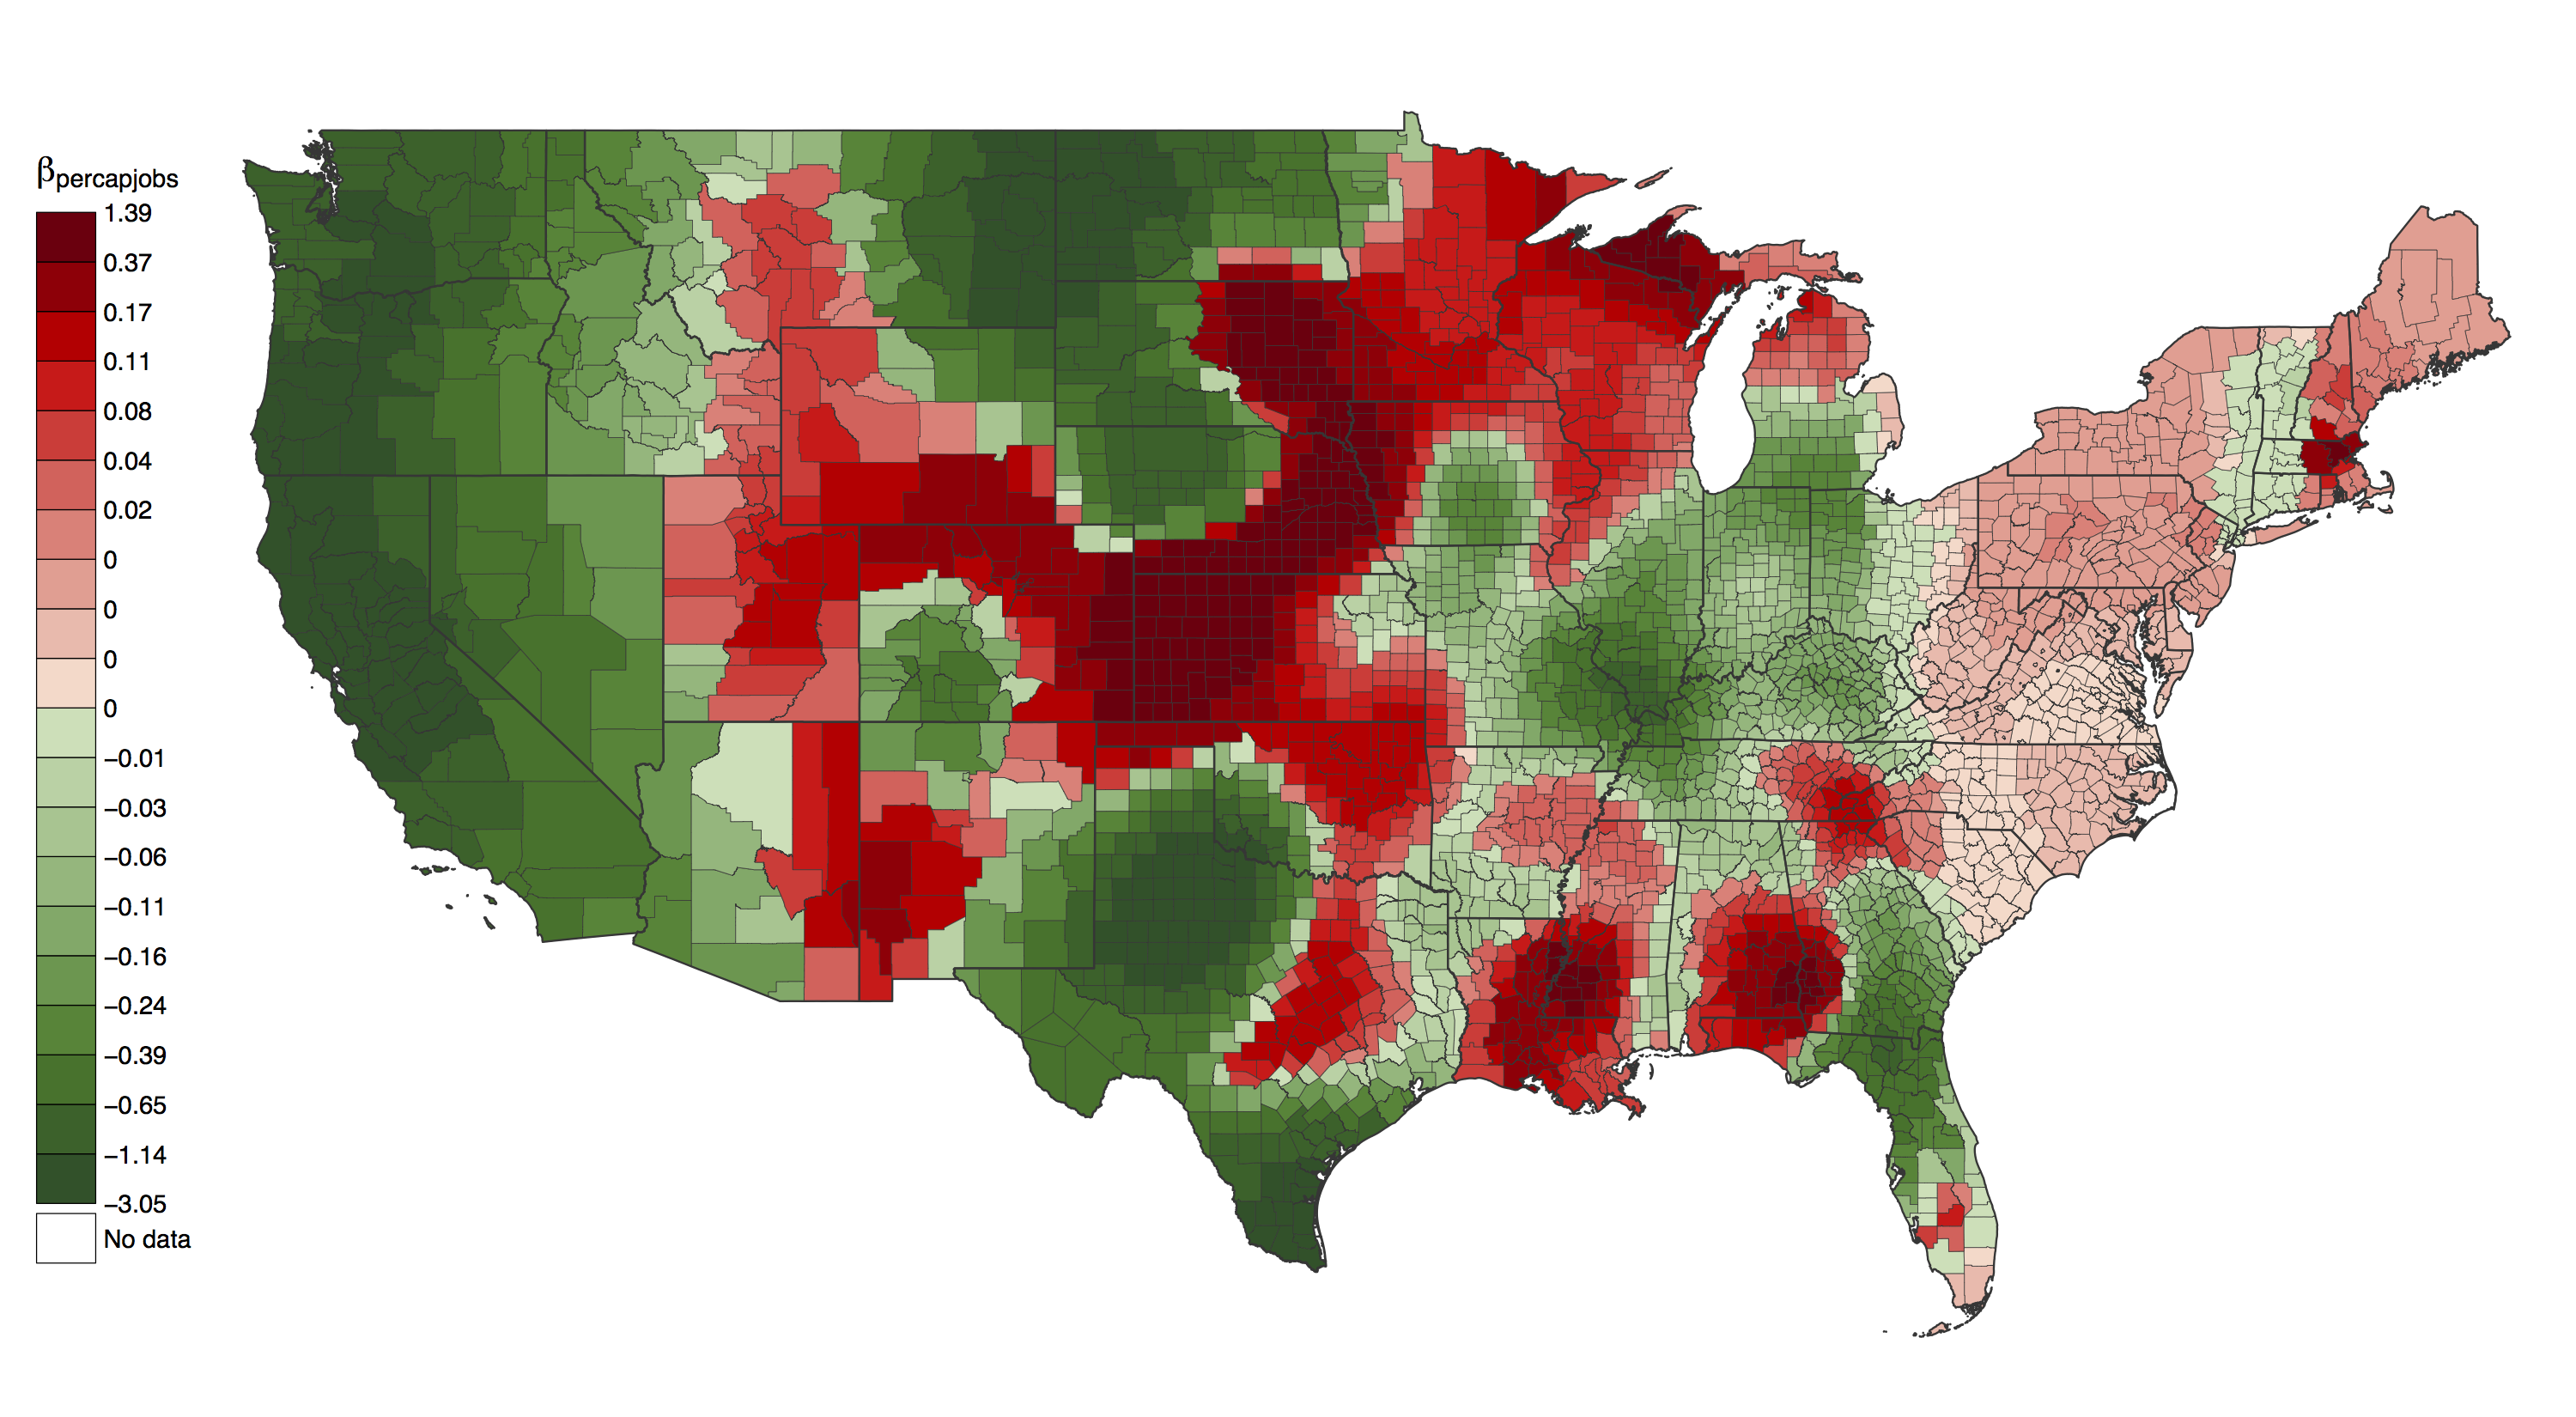
\includegraphics[width=0.48\textwidth]{figures/gwr_allbest_betapercapjobs}\\
%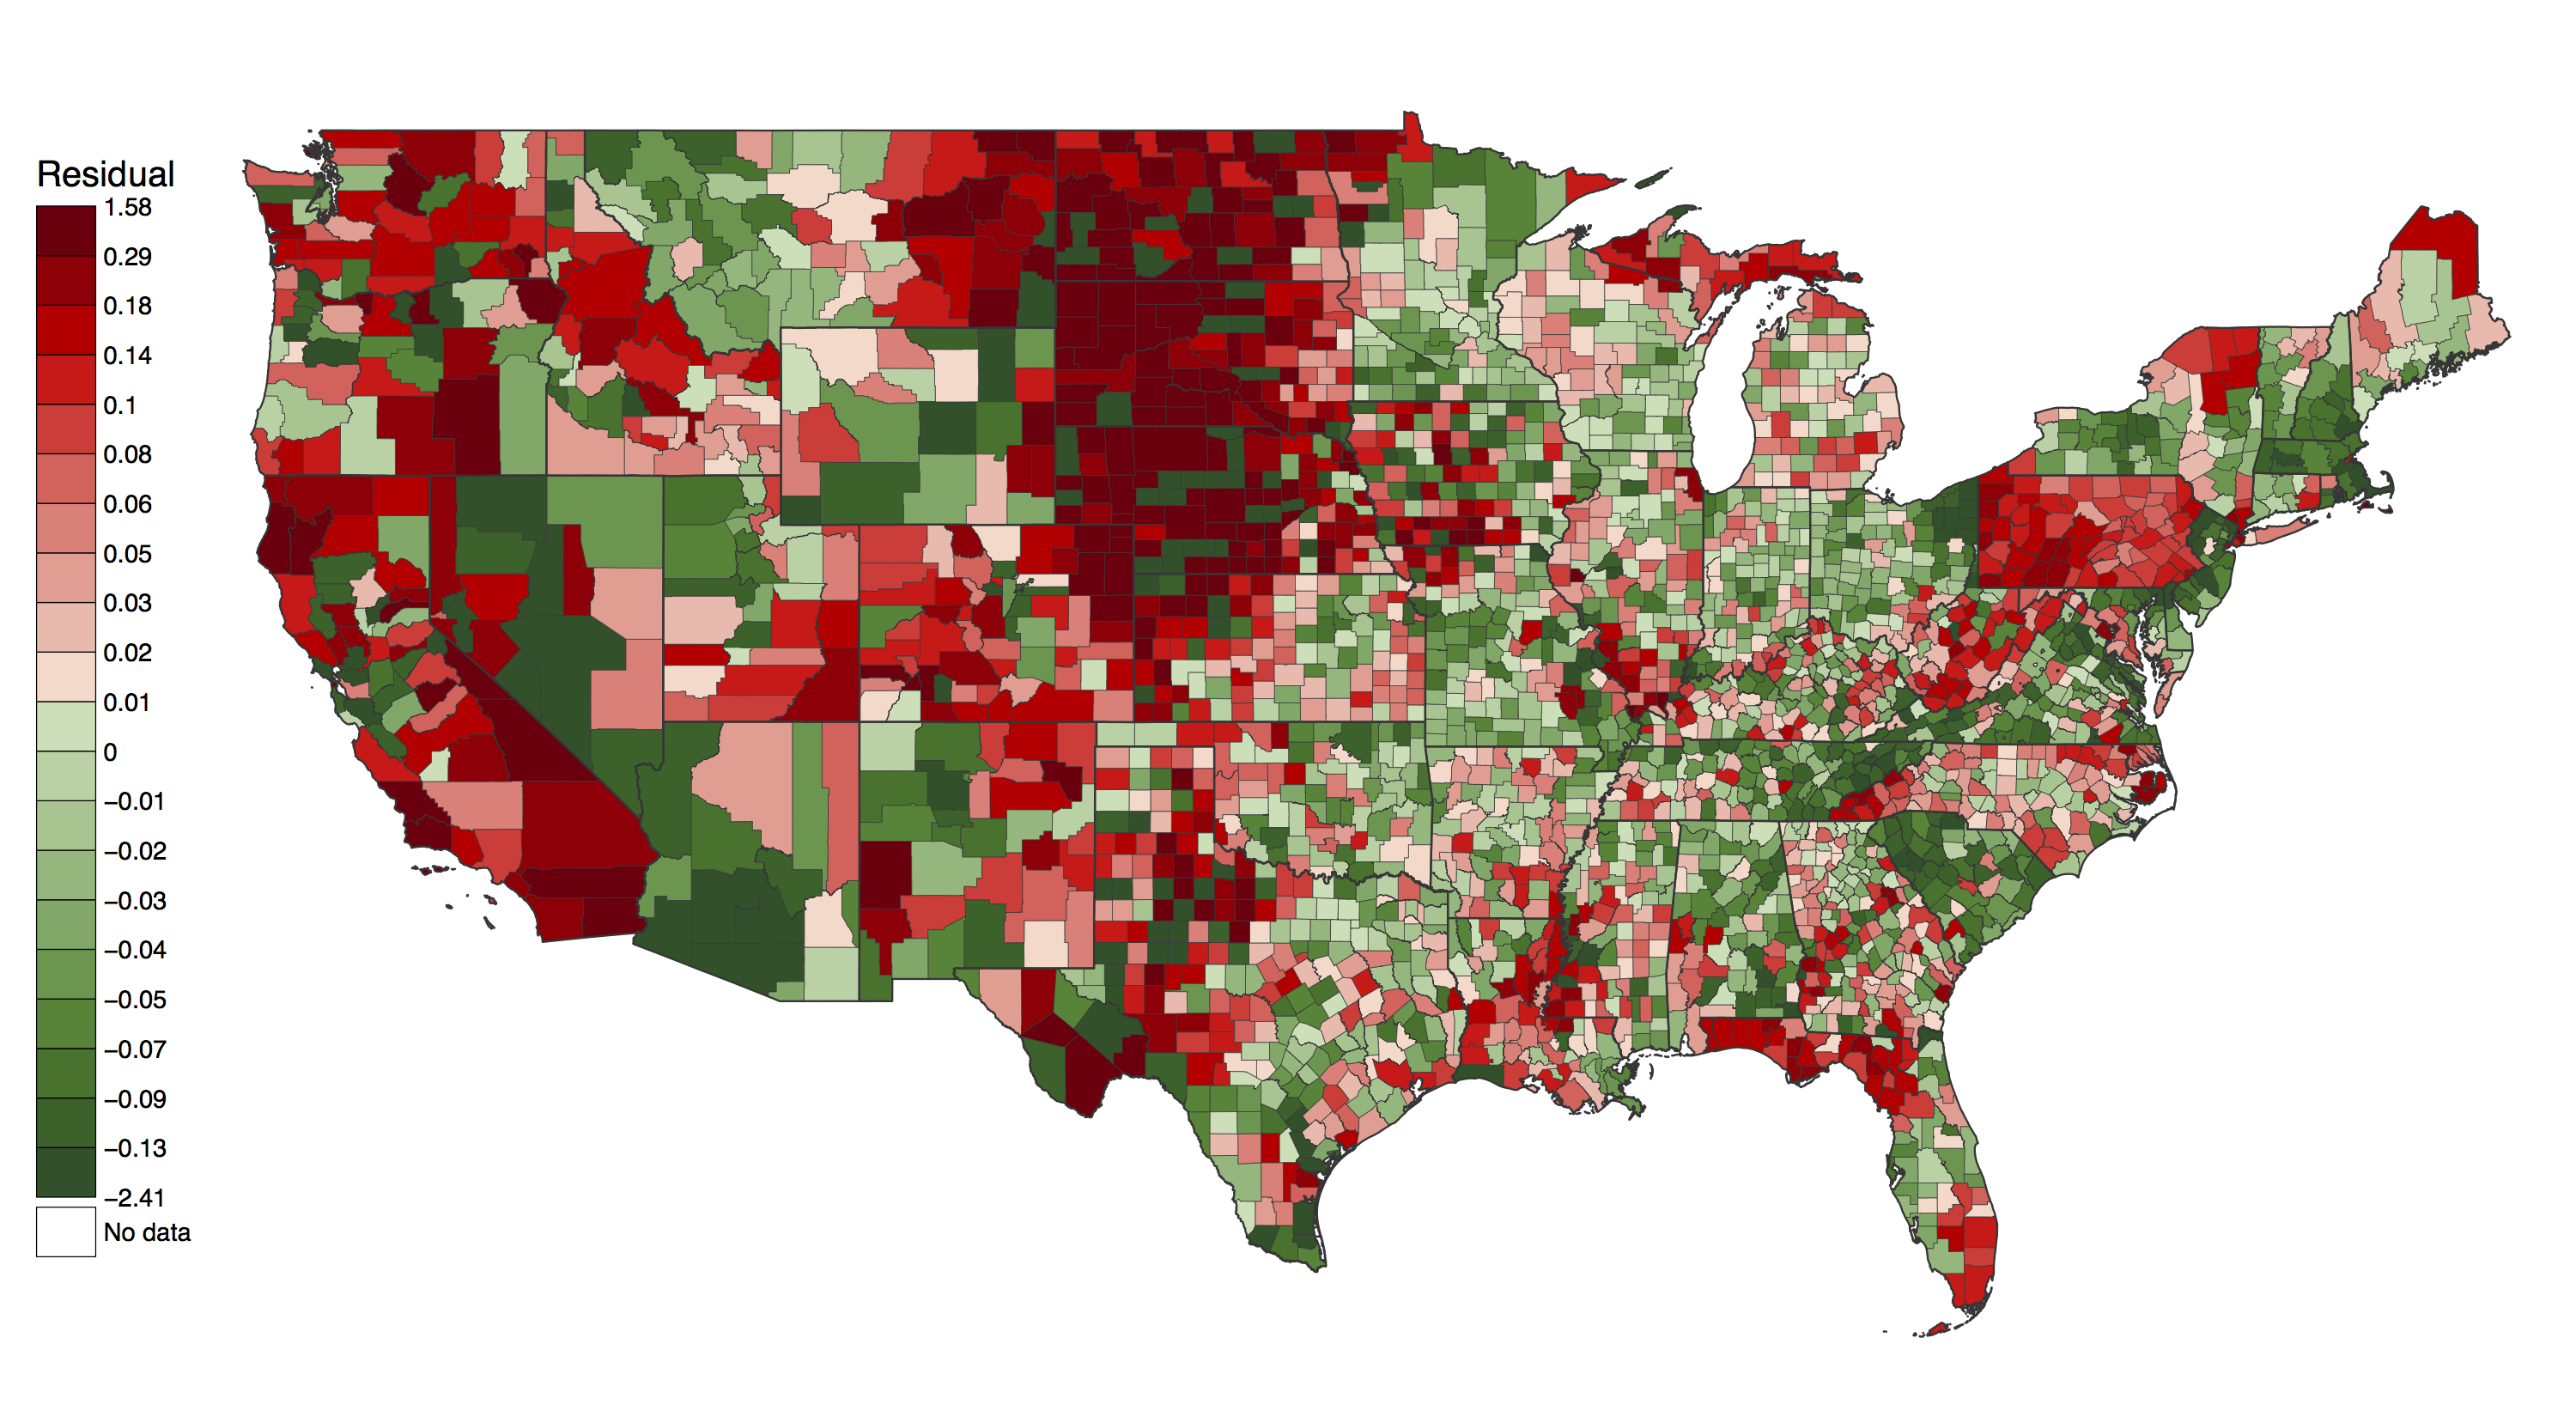
\includegraphics[width=0.48\textwidth]{figures/gwr_allbest_residual}
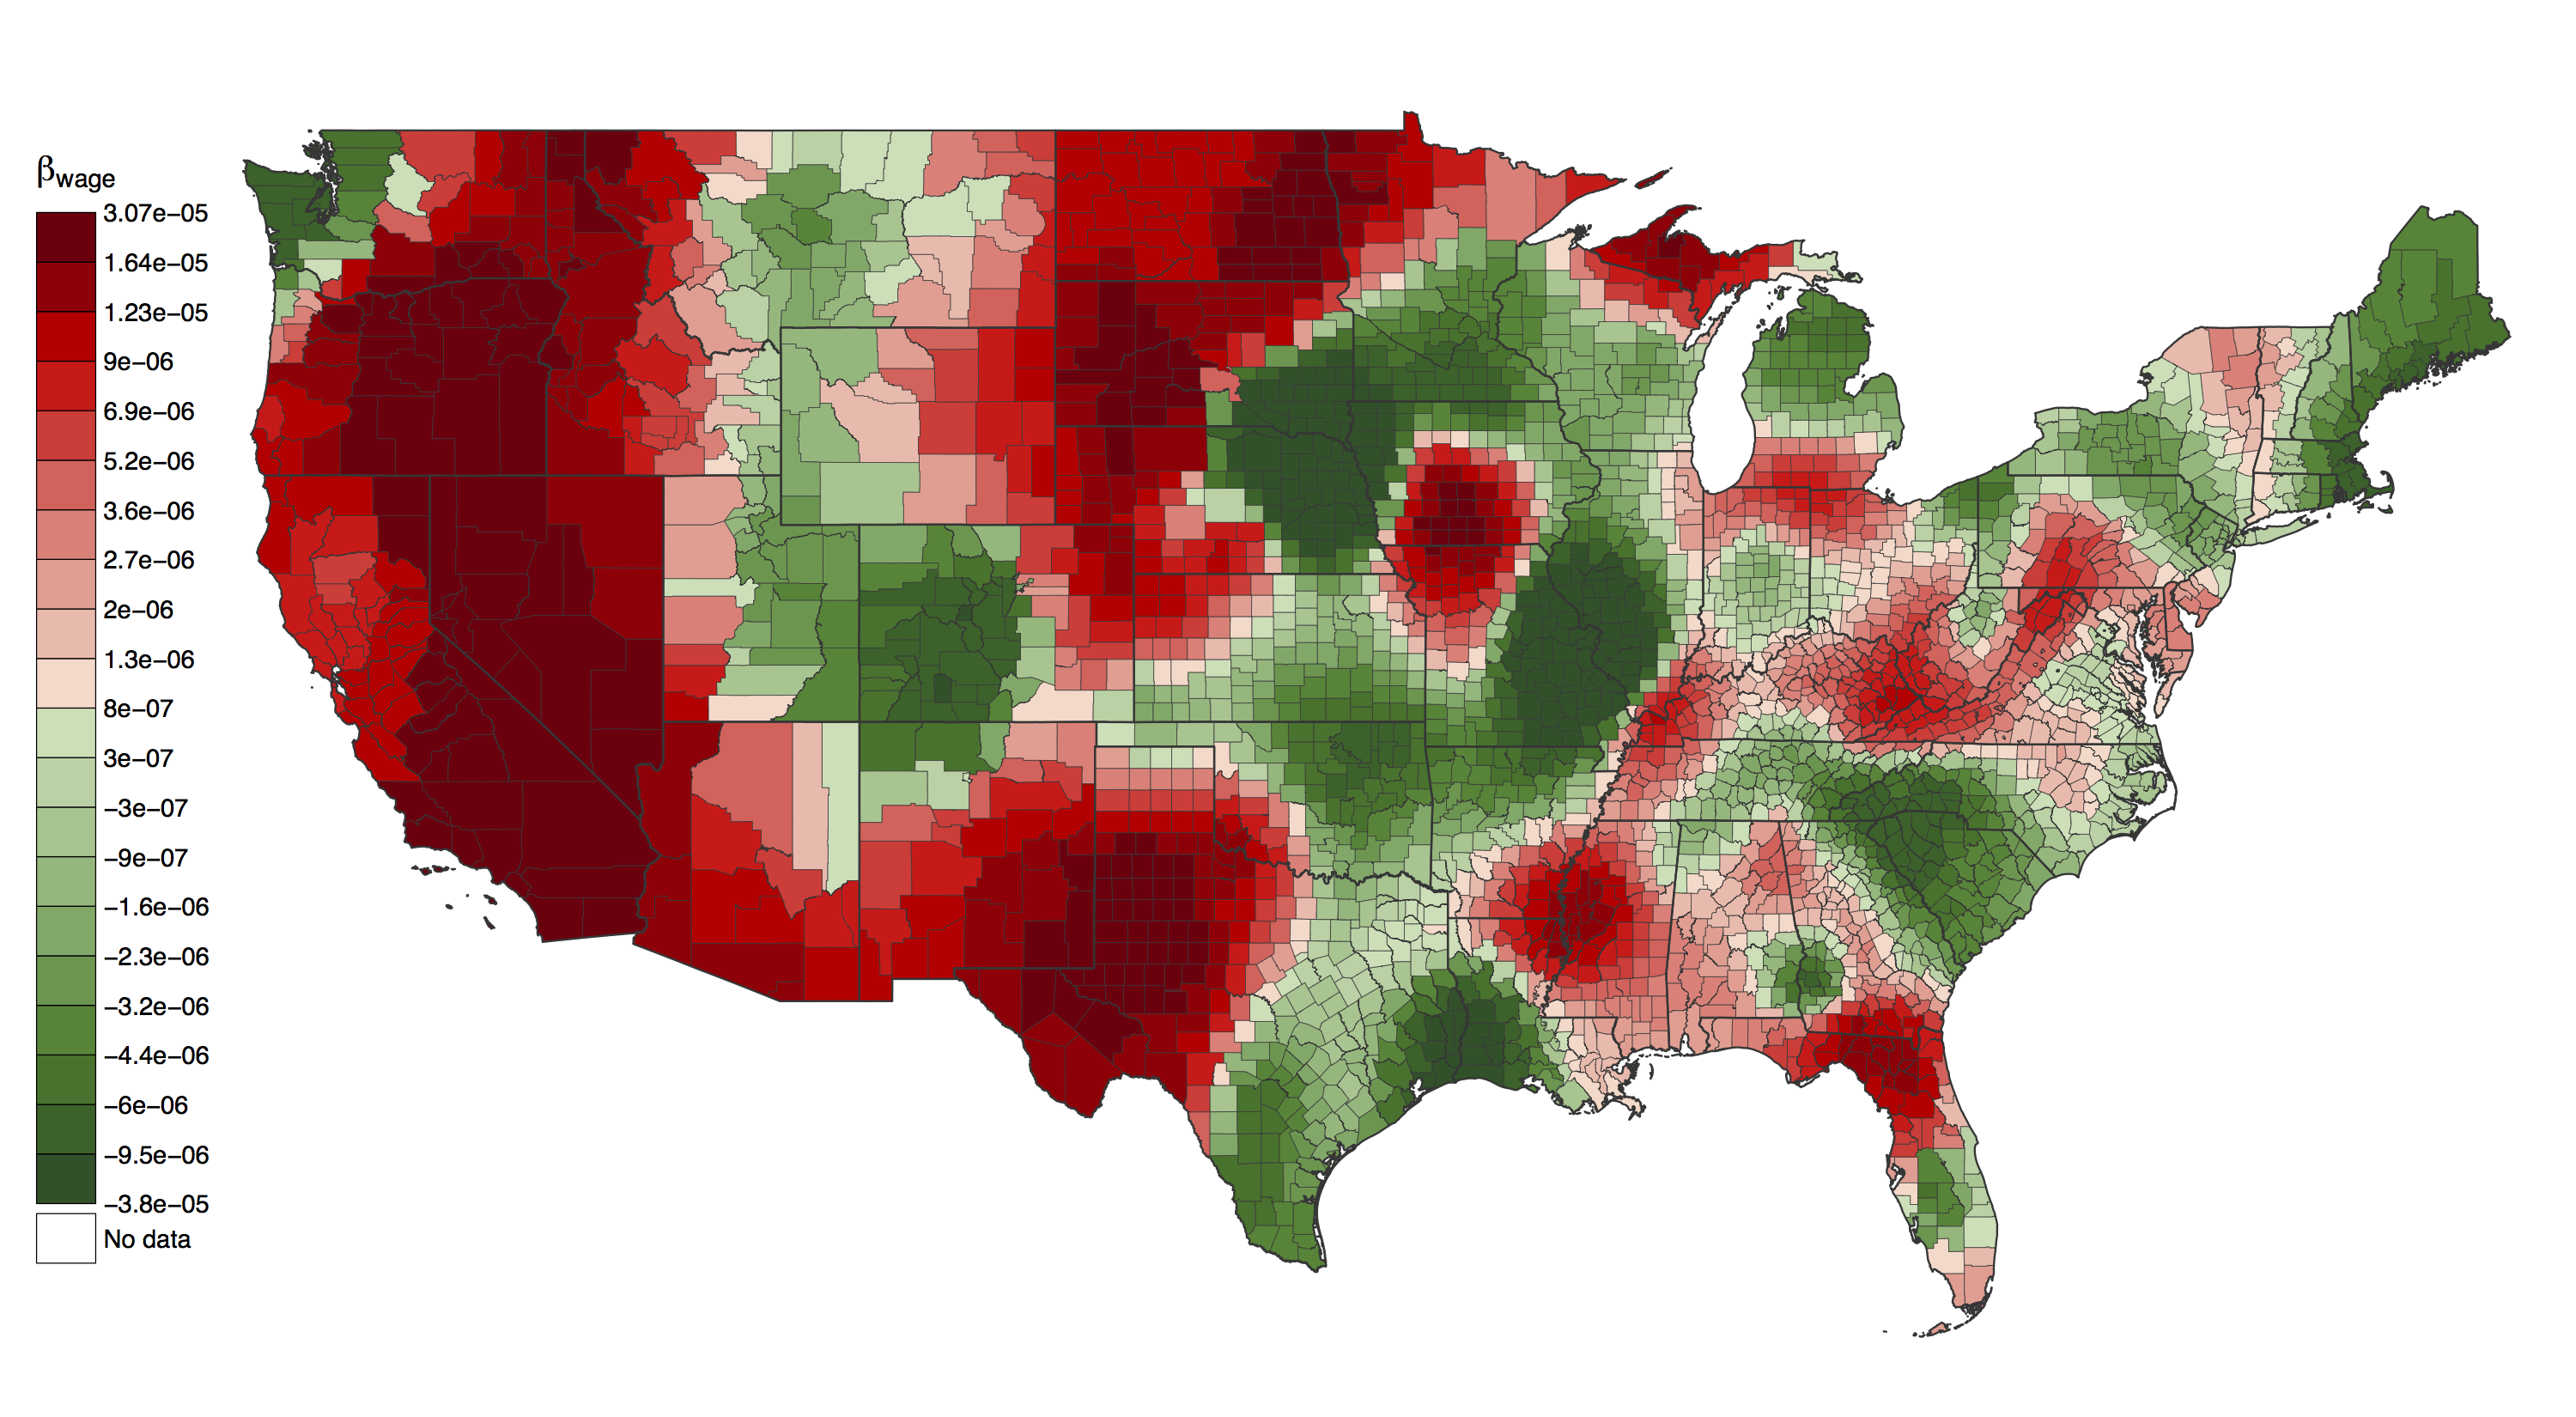
\includegraphics[width=0.48\textwidth]{figures/gwr_allbest_wage}
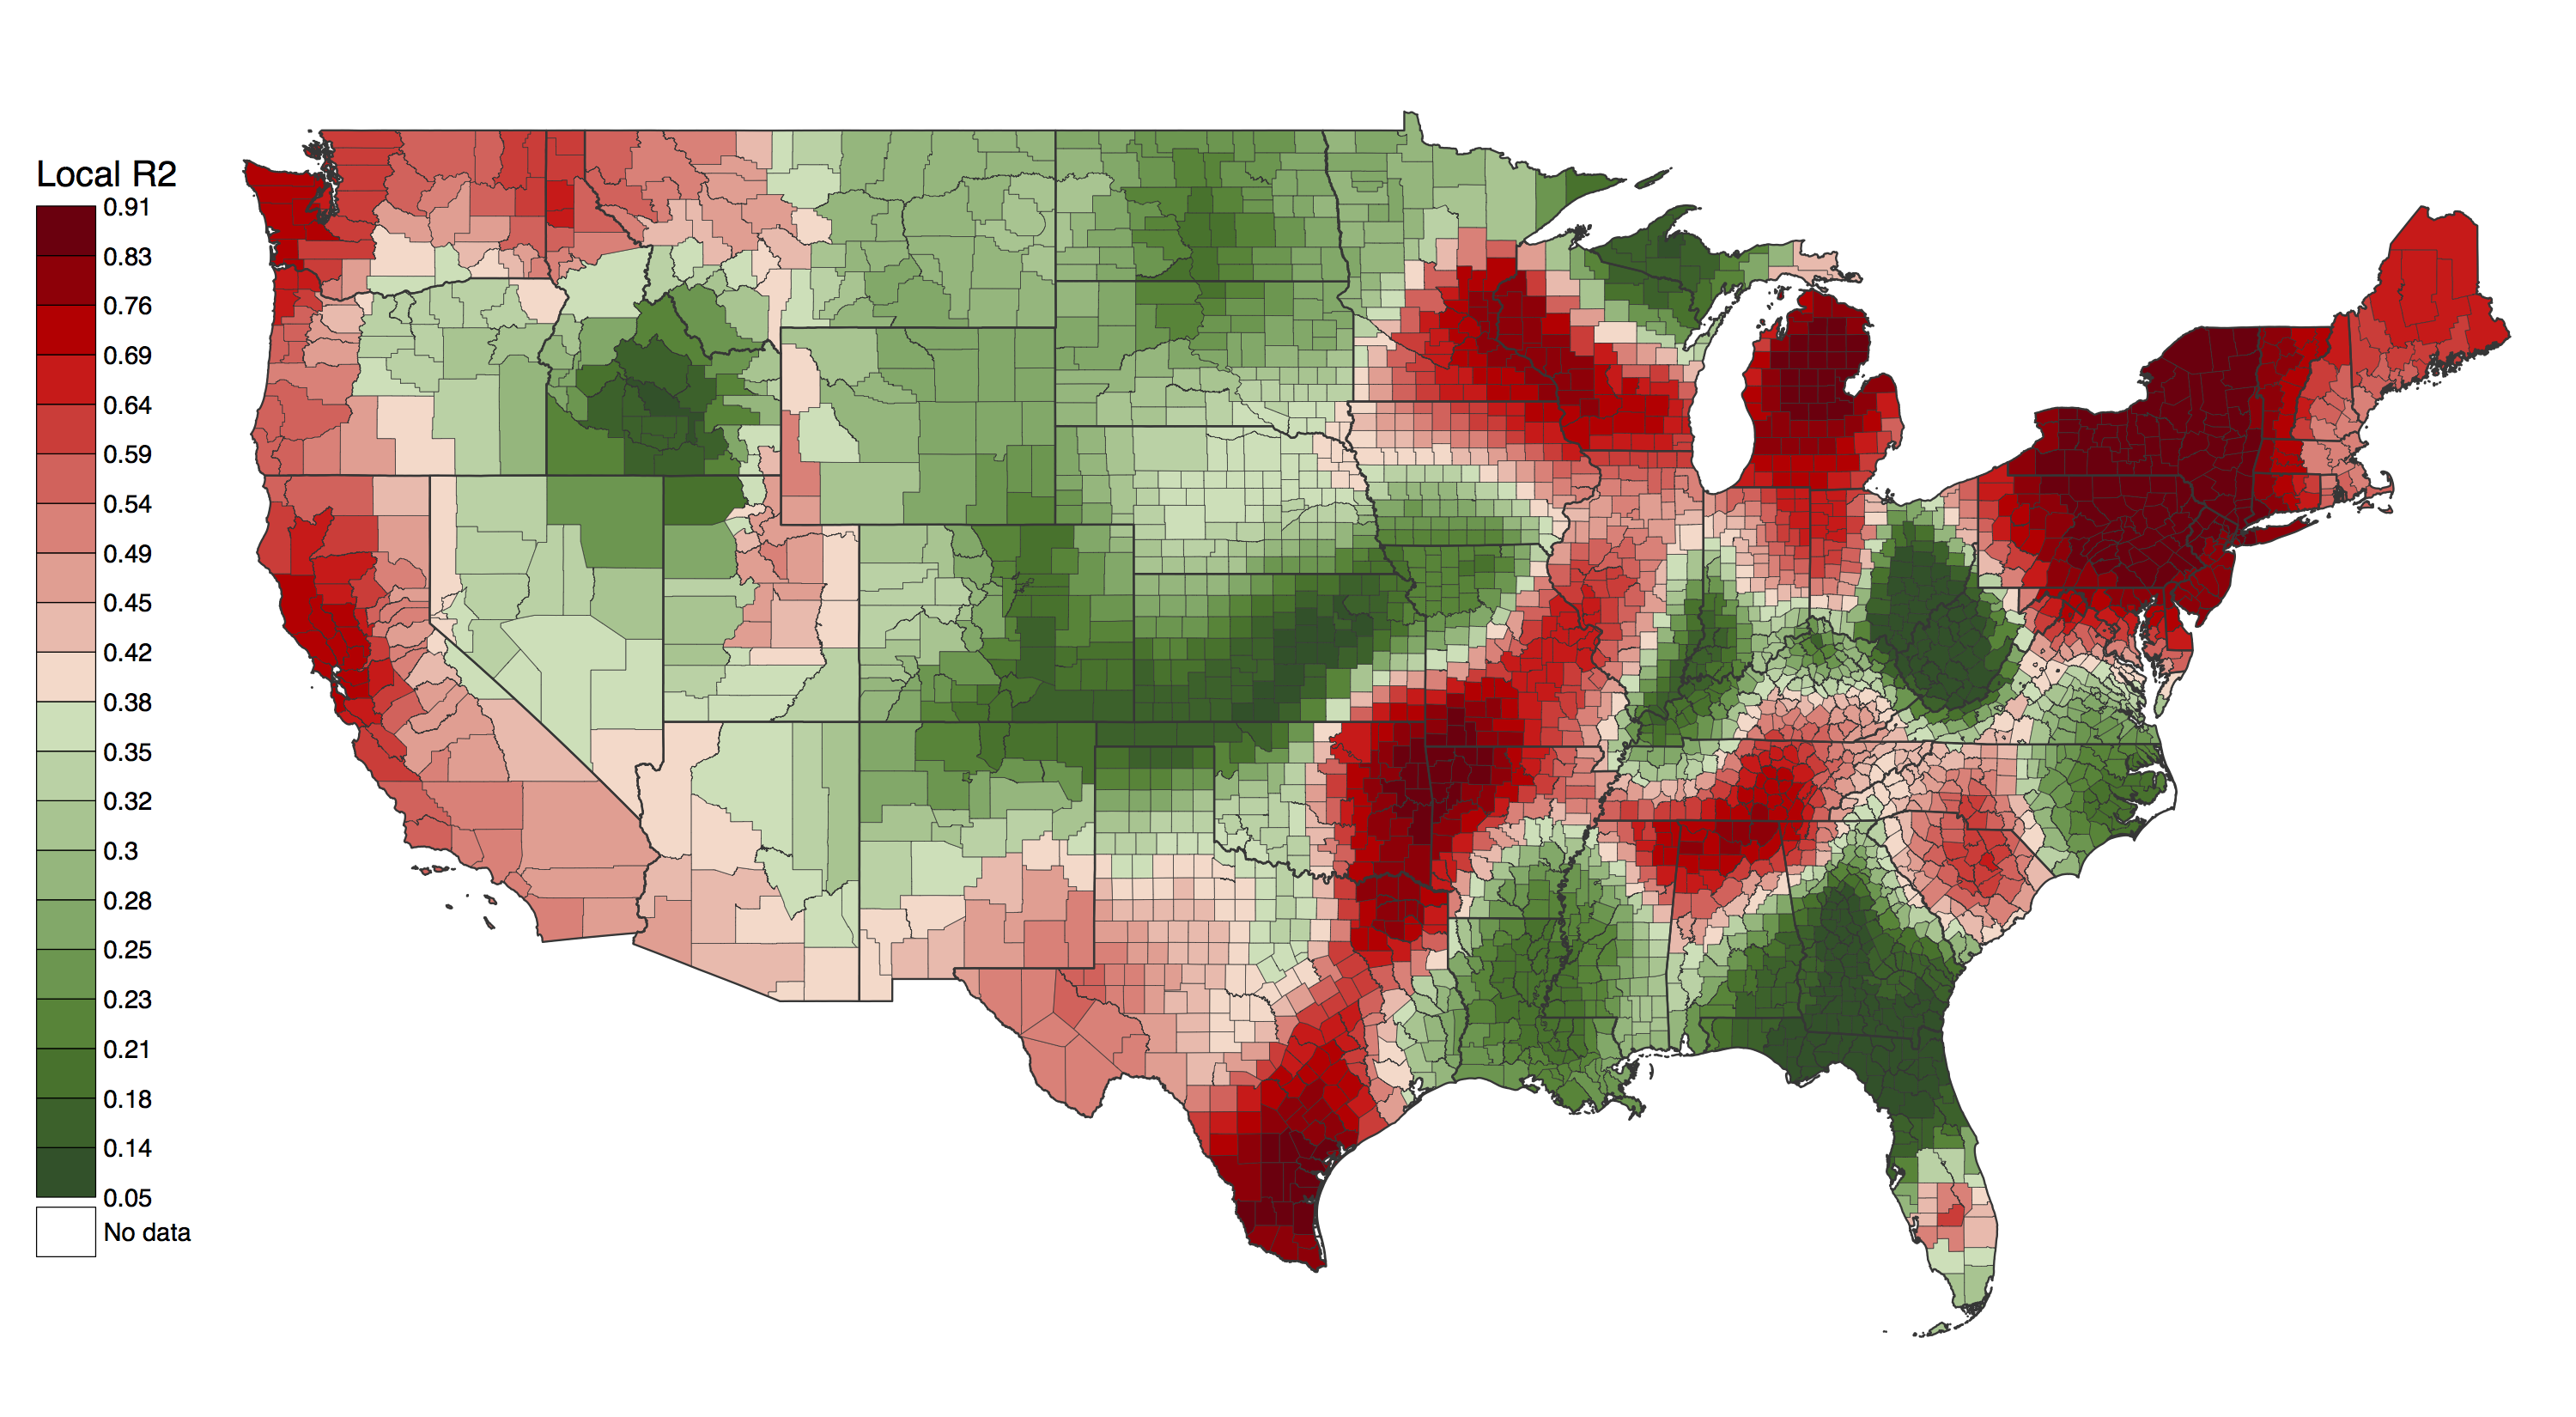
\includegraphics[width=0.48\textwidth]{figures/gwr_allbest_LocalR2}
\caption{\textbf{Results of GWR analyses.} For the best model in the sense of AICc, we map the spatial distribution of fitted coefficient, in order from left to right and top to bottom, $\beta_{income}$, $\beta_{percapjobs}$, $\beta_{wage}$}
\label{fig:gwr}
\end{figure}
%%%%%%%%%%%%%%%%%%%%%%


%%%%%%%%%%%%%%%%%%%%%%
\subsection{Multi-level Regression}

An other approach to take into account geographical heterogeneities without explicitly including spatial relations between objects is to proceed to regressions with random effects depending on geographical aggregations at different levels. The method of multi-level regression implements this idea, and has been shown to be particularly adapted for geographical research~\cite{jones1991specifying}. We take here into account two administrative levels, the state and the county. Explorations of section~\ref{subsec:patterns} suggest a strong state-effect that GWR cannot capture around boundaries, what confirms the relevance and complementarity of using Multi-level Regression.






%%%%%%%%%%%%%%%%%%%%%%
\section{Discussion} \label{sec:discuss}
%%%%%%%%%%%%%%%%%%%%%%

\subsection{On the complementarity on Spatial Analysis methods}

\comment{bla bla on conclusions drawn with each method ; how they are complementary $\rightarrow$ also present it as a methodological contribution. some literature do both, e.g. Chen, D. R., \& Truong, K. (2012). Using multilevel modeling and geographically weighted regression to identify spatial variations in the relationship between place-level disadvantages and obesity in Taiwan. Applied Geography, 32(2), 737-745. integrates both in a single approach.}


\subsection{Towards localized car-regulation policies}

% local energy taxing ?
\comment{knowing local price dynamics and their drivers should help designing specific regulations/taxing policies ?}


%%%%%%%%%%%%%%%%%%%%%%
\section{Conclusion}






%\section*{Acknowledgements}

%Acknowledgements and Reference heading should be left justified, bold, with the first letter capitalized but have no numbers. Text below continues as normal.

%% The Appendices part is started with the command \appendix;
%% appendix sections are then done as normal sections
%% \appendix

%% \section{}
%% \label{}



%% References
%%
%% Following citation commands can be used in the body text:
%% Usage of \cite is as follows:
%%   \cite{key}         ==>>  [#]
%%   \cite[chap. 2]{key} ==>> [#, chap. 2]
%%

%The citation must be used in following style: \cite{article-minimal} \cite{article-full} \cite{article-crossref} \cite{whole-journal}.
%% References with BibTeX database:


\bibliographystyle{elsarticle-harv}
\bibliography{biblio}
%


\clearpage
\end{document}

%%
%% End of file `procs-template.tex'.


%%%%%%%%%%%%%%%%%%%
%%  TEMPLATES


%
%Here introduce the paper, and put a nome¬nclature if necessary, in a box with the same font size as the rest of the paper. The paragraphs continue from here and are only separated by headings, subheadings, images and formulae. The section headings are arranged by numbers, bold and 10 pt. Here follows further instructions for authors.
%
%\begin{nomenclature}
%\begin{deflist}[A]
%\defitem{A}\defterm{radius of}
%\defitem{B}\defterm{position of}
%\defitem{C}\defterm{further nomenclature continues down the page inside the text box\vspace*{-8pt}}
%\end{deflist}
%\end{nomenclature}
%\vspace*{0pt}
%
%\subsection{Structure}
%Files must be in LaTeX format only and should be formatted for direct printing, using the CRC LaTeX template provided. Figures and tables should be embedded and not supplied separately. 
%
%Please make sure that you use as much as possible normal fonts in your documents. Special fonts, such as fonts used in the Far East (Japanese, Chinese, Korean, etc.) may cause problems during processing. To avoid unnecessary errors you are strongly advised to use the `spellchecker' function of TeX Editor. Follow this order when typing manuscripts: Title, Authors, Affiliations, Abstract, Keywords, Main text (including figures and tables), Acknowledgements, References, Appendix. Collate acknowledgements in a separate section at the end of the article and do not include them on the title page, as a footnote to the title or otherwise.
%
%Bulleted lists may be included and should look like this:
%\begin{itemize}[]
%\item First point
%\item Second point
%\item And so on
%\end{itemize}
%
%Ensure that you return to the `Els-body-text' style, the style that you will mainly be using for large blocks of text, when you have completed your bulleted list. 
%
%Please do not alter the formatting and style layouts which have been set up in this template document. As indicated in the template, papers should be prepared in single column format suitable for direct printing onto paper with trim size $192 \times 262$ mm. Do not number pages on the front, as page numbers will be added separately for the preprints and the Proceedings. Leave a line clear between paragraphs. All the required style templates are provided in the file ``LaTeX Template'' with the appropriate name supplied, e.g. choose 1. Els1st-order-head for your first order heading text, els-abstract-text for the abstract text etc.
%
%\subsection{ Tables}
%
%All tables should be numbered with Arabic numerals. Every table should have a caption. Headings should be placed above tables, left justified. Only horizontal lines should be used within a table, to distinguish the column headings from the body of the table, and immediately above and below the table. Tables must be embedded into the text and not supplied separately. Below is an example which the authors may find useful.
%
%\begin{table}[h]
%\caption{An example of a table.}
%\begin{tabular*}{\hsize}{@{\extracolsep{\fill}}lll@{}}
%\toprule
%An example of a column heading & Column A ({\it{t}}) & Column B ({\it{t}})\\
%\colrule
%And an entry &   1 &  2\\
%And another entry  & 3 &  4\\
%And another entry &  5 &  6\\
%\botrule
%\end{tabular*}
%\end{table}
%
%%\enlargethispage{12pt}
%
%\subsection{ Construction of references}
%
%References must be listed at the end of the paper. Do not begin them on a new page unless this is absolutely necessary. Authors should ensure that every reference in the text appears in the list of references and vice versa. Indicate references by \cite{clark} or \cite{Deal} or \cite{Fachinger2006} in the text. 
%
%Some examples of how your references should be listed are given at the end of this template in the `References' section, which will allow you to assemble your reference list according to the correct format and font size.
%
%Reference generation by using bibliography style commands for LaTeX template only.
%
%The author may use ``elsarticle-harv.bst'' as per the style required in document. The sample bib file could be referred. 
%If the author may using bibstyle for providing references author must comment the bibliography section in TeX file, Bibtex will generate the reference automatically.
%
%If the author may not able to view the references in output same could be done by copying the bibliography section from ``filename.bbl'' file and paste in TeX file.
%
%
%
%\subsection{Section headings}
%Section headings should be left justified, bold, with the first letter capitalized and numbered consecutively, starting with the Introduction. Sub-section headings should be in capital and lower-case italic letters, numbered 1.1, 1.2, etc,~and left justified, with second~and subsequent lines indented. All headings should have a minimum of two text lines after them before a page or column break.
%Ensure the text area is not blank except for the last page.
%
%\subsection{General guidelines for the preparation of your text}
%Avoid hyphenation at the end of a line. Symbols denoting vectors and matrices should be indicated in bold type. Scalar variable names should normally be expressed using italics. Weights and measures should be expressed in SI units. All non-standard abbreviations or symbols must be defined when first mentioned, or a glossary provided.
%
%\subsection{File naming and delivery}
%Please title your files in this order `procedia acronym\_conference acronym\_authorslastname'.  Submit both the source file and the PDF to the Guest Editor.
%
%Artwork filenames should comply with the syntax ``aabbbbbb.ccc'', where:\vspace*{-12pt}
%\begin{itemize}
%\item a = artwork component type
%\item b = manuscript reference code
%\item c = standard file extension
%
%Component types:
%\item gr = figure
%\item pl = plate
%\item sc = scheme
%\item fx = fixed graphic
%\end{itemize}



%
%
%
%\subsection{Footnotes}
%Footnotes should be avoided if possible. Necessary footnotes should be denoted in the text by consecutive superscript letters\footnote{Footnote text.}. The footnotes should be typed single spaced, and in smaller type size (8 pt), at the foot of the page in which they are mentioned, and separated from the main text by a one line space extending at the foot of the column. The `Els-footnote' style is available in the ``TeX Template'' for the text of the footnote.
%
%Please do not change the margins of the template as this can result in the footnote falling outside printing range.
%
%
%\section{Illustrations}
%All figures should be numbered with Arabic numerals (1,2,3,\,$\ldots.$). Every figure should have a caption. All\break photographs, schemas, graphs and diagrams are to be referred to as figures. Line drawings should be good quality\break scans or true electronic output. Low-quality scans are not acceptable. Figures must be embedded into the text and not supplied separately. In MS word input the figures must be properly coded. Preferred format of figures are PNG, JPEG, GIF etc. Lettering and symbols should be clearly defined either in the caption or in a legend provided as part of the figure. Figures should be placed at the top or bottom of a page wherever possible, as close as possible to the first reference to them in the paper. Please ensure that all the figures are of 300 DPI resolutions as this will facilitate good output.
%\begin{figure}[t]\vspace*{4pt}
%%\centerline{\includegraphics{fx1}\hspace*{5mm}\includegraphics{fx1}}
%\centerline{\includegraphics{gr1}}
%\caption{(a) first picture; (b) second picture.}
%\end{figure}
%
%The figure number and caption should be typed below the illustration in 8 pt and left justified [{{\bfseries\itshape Note:}} one-line captions of length less than column width (or full typesetting width or oblong) centered]. For more guidelines and information to help you submit high quality artwork please visit: http://www.elsevier.com/artworkinstructions\break Artwork has no text along the side of it in the main body of the text. However, if two images fit next to each other, these may be placed next to each other to save space. For example, see Fig.~1. 
%
%
%\section{Equations}
%Equations and formulae should be typed in Mathtype, and numbered consecutively with Arabic numerals in parentheses on the right hand side of the page (if referred to explicitly in the text). They should also be separated from the surrounding text by one space
%\begin{equation}
%\begin{array}{lcl}
%\displaystyle X_r &=& \displaystyle\dot{Q}^{''}_{rad}\left/\left(\dot{Q}^{''}_{rad} + \dot{Q}^{''}_{conv}\right)\right.\\[6pt]
%\displaystyle \rho &=& \displaystyle\frac{\vec{E}}{J_c(T={\rm const.})\cdot\left(P\cdot\left(\displaystyle\frac{\vec{E}}{E_c}\right)^m+(1-P)\right)}
%\end{array}
%\end{equation}
%
%
%\section{Online license transfer}
%All authors are required to complete the Procedia exclusive license transfer agreement before the article can be published, which they can do online. This transfer agreement enables Elsevier to protect the copyrighted material for the authors, but does not relinquish the authors' proprietary rights. The copyright transfer covers the exclusive rights to reproduce and distribute the article, including reprints, photographic reproductions, microfilm or any other reproductions of similar nature and translations. Authors are responsible for obtaining from the copyright holder, the permission to reproduce any figures for which copyright exists.
%

%
%
%\appendix
%\section{An example appendix}
%Authors including an appendix section should do so before References section. Multiple appendices should all have headings in the style used above. They will automatically be ordered A, B, C etc.
%
%\subsection{Example of a sub-heading within an appendix}
%There is also the option to include a subheading within the Appendix if you wish.
%



%% Authors are advised to use a BibTeX database file for their reference list.
%% The provided style file elsarticle-num.bst formats references in the required Procedia style

%% For references without a BibTeX database:

% \begin{thebibliography}{}
%
%%% \bibitem must have the following form:
%%%   \bibitem{key}...
%%%
%
%\bibitem[Clark et al.(1962)]{clark}Clark, T., Woodley, R., De Halas, D., 1962. Gas-Graphite Systems, in ``{\it Nuclear Graphite}''. 
%In: Nightingale, R. (Ed.). Academic Press, New York, pp. 387.
%
%\bibitem[Deal and Grove(2009) ]{Deal}Deal, B., Grove, A., 1965. General Relationship for the Thermal Oxidation of Silicon. Journal of Applied Physics 36, 37--70.
%
%\bibitem[Deep(2009)]{Deep}Deep-Burn Project: Annual Report for 2009, Idaho National Laboratory, Sept. 2009.
%
%\bibitem[Fachinger(2004)]{Fachinger2004}Fachinger, J., den Exter, M., Grambow, B., Holgerson, S., Landesmann, C., Titov, M., Podruhzina, T., 2004. ``Behavior of spent HTR fuel elements in aquatic phases of repository host rock formations,'' 2nd International Topical Meeting on High Temperature Reactor Technology. Beijing, China, paper \#B08. 
%
%\bibitem[Fachinger(2006)]{Fachinger2006}Fachinger, J., 2006. Behavior of HTR Fuel Elements in Aquatic Phases of Repository Host Rock Formations. Nuclear Engineering \& Design 236,     54.
%
%
% \end{thebibliography}
%

%
%
%%%%% This page is for instructions only, once the article is finalize please omit the below text before creating the final PDF
%\normalMode
%
%\section*{Instructions to Authors for LaTeX template:}
%
%\section{ZIP mode for LaTeX template:}
%
%The zip package is created as per the guide lines present on the URL http://www.elsevier.com/author-schemas/ preparing-crc-journal-articles-with-latex for creating the LaTeX zip file of Procedia LaTeX template.  The zip generally contains the following files:
%\begin{Itemize}[]\leftskip-17.7pt\labelsep3.3pt
%\item ecrc.sty
%\item  elsarticle.cls
%\item elsdoc.pdf
%\item .bst file
%\item Manuscript templates for use with these bibliographic styles
%\item  Generic and journal specific logos, etc.
%\end{Itemize}
%
%The LaTeX package is the main LaTeX template. All LaTeX support files are required for LaTeX pdf generation from the LaTeX template package. 
%
%{\bf Reference style .bst file used for collaboration support:} In the LaTeX template packages of all Procedia titles a new ``.bst'' file is used which supports collaborations downloaded from the path http://www.elsevier.com/author-schemas/the-elsarticle-latex-document-class
%
%\section{Reference styles used in  Procedia master templates:}
%\let\footnotesize\normalsize
%\hspace*{-10pt}\begin{tabular*}{\hsize}{@{}ll@{}}
%{\bf Title}&{\bf Reference style} \\[6pt]
%AASPRO  & 2 Harvard\\
%AASRI Procedia  & 3 Vancouver Numbered\\
%APCBEE Procedia  & 3 Vancouver Numbered\\
%EGYPRO  & 3 Vancouver Numbered\\
%FINE    & 2 Harvard\\
%IERI Procedia  & 3 Vancouver Numbered\\
%MATPR  & 1a Numbered without article titles\\
%MSPRO  & 2 Harvard\\
%PHPRO  & 2 Harvard\\
%PIUTAM  & 3a Embellished Vancouver \\
%Procedia CIRP  & 3 Vancouver Numbered\\
%PROCHE  & 3a Embellished Vancouver \\
%PROCS  & 3a Embellished Vancouver \\
%PROENG  & 1 Numbered\\
%PROENV  & 3a Embellished Vancouver \\
%PROEPS  & 3a Embellished Vancouver \\
%PROFOO    & 3a Embellished Vancouver \\
%PROMFG  & 1a Numbered without article titles\\
%PROTCY  & 3 Vancouver Numbered\\
%PROVAC  & 3a Embellished Vancouver \\
%SBSPRO  & 5 APA\\
%SEPRO  & 3a Embellished Vancouver \\
%AQPRO & 2 Harvard\\
%UMKPRO & 5 APA\\
%TRPRO  & 2 Harvard\\
%\end{tabular*}
%






